\documentclass[t]{beamer}

% Load general definitions
% Preamble file - general definitions, package loading, etc.

%=================================
% Load packages
\usepackage{amssymb,amsmath}
\usepackage{graphicx}
\usepackage{url}
\usepackage{tikz}
\usetikzlibrary{mindmap,trees,arrows}
\usepackage{fancyvrb}
\usepackage[portuguese]{babel} 
\usepackage[utf8]{inputenc}
\usepackage{subfigure}
\usepackage{times}
\usepackage[T1]{fontenc}
\usepackage{cancel}
\usepackage{color}
\usepackage{listings}
\usepackage[document]{ragged2e}
\usepackage{physics}
\usepackage{amsmath}
\usepackage{tikz}
\usepackage{mathdots}
\usepackage{yhmath}
\usepackage{cancel}
\usepackage{color}
\usepackage{siunitx}
\usepackage{array}
\usepackage{multirow}
\usepackage{amssymb}
\usepackage{gensymb}
\usepackage{tabularx}
\usepackage{extarrows}
\usepackage{booktabs}
\usetikzlibrary{fadings}
\usetikzlibrary{patterns}
\usetikzlibrary{shadows.blur}
\usetikzlibrary{shapes}

%=================================
% Set mode
\mode<presentation>
{
	\usetheme{Madrid}
	\usecolortheme{structure}
	\useoutertheme{infolines}
	\setbeamercovered{invisible}
}

% Get rid of nav bar
\beamertemplatenavigationsymbolsempty

% Insert frame number at bottom of the page.
\usefoottemplate{\hfil\tiny{\color{black!90}\insertframenumber}} 

%=================================
% Define new commands

\newcommand\Real{{\mathbb{R}}}
%\newcommand{\vi}{\vspace{0.6\baselineskip}}
%\newcommand{\goodgap}{\hspace{\subfigtopskip}\hspace{\subfigbottomskip}}


% Equation environments
\newcommand{\beq}{\begin{equation}}
\newcommand{\eq}{\end{equation}}
\newcommand{\beqs}{\begin{equation*}}
\newcommand{\eqs}{\end{equation*}}
\newcommand{\beqn}{\begin{eqnarray}}
\newcommand{\eqn}{\end{eqnarray}}
% Bold variables
\newcommand{\mbf}[1]{\ensuremath{\mathbf{#1}}}
% Itemization
\newcommand{\bitem}{\begin{itemize}}
\newcommand{\eitem}{\end{itemize}}
\newcommand{\spitem}{\vskip 1em\item}
\newcommand{\bitems}{\begin{itemize}\item}
\newcommand{\benums}{\begin{enumerate}\item}
\newcommand{\eenum}{\end{enumerate}}
% color blocks
\newenvironment{colorblock}[2]{%
\setbeamercolor{block title}{#2}
\begin{block}{#1}}{\end{block}}
% Vertical spacing
\newcommand{\vone}{\vskip 1em}
\newcommand{\vhalf}{\vskip .5em}
% Frame environments
\newenvironment{ftst}[3][t]{%
\begin{frame}{environment=ftst,#1}
\frametitle{#2}
\framesubtitle{#3}}{\end{frame}}
\newenvironment{ftstf}[2]{
\begin{frame}[fragile,environment=ftstf]
\frametitle{#1}
\framesubtitle{#2}}{\end{frame}}
% colors
\definecolor{MyGray}{rgb}{0.5,0.5,0.5}
\definecolor{MyDBGray}{rgb}{0.1,0.1,0.4}
\definecolor{darkgreen}{rgb}{0,0.4,0}
\definecolor{black}{rgb}{0,0,0}
\def\defn#1{{\color{red} #1}}
% Footnote
\renewcommand{\thefootnote}{\alph{footnote}}
% Relaxed footnotes
\newcommand{\lfr}[1]{\let\thefootnote\relax\footnote{\tiny #1}}
% Verbatim environment - using FANCYVRB package
\DefineVerbatimEnvironment%
{rcode}{Verbatim}
{fontsize=\scriptsize}
% Verbatim environment - using LISTINGS package
%\lstnewenvironment{rcode} {\lstset{	language = R,
%									basicstyle = \scriptsize\ttfamily,
%									showspaces = false,
%									showstringspaces = false,
%									showtabs = false,
%									keywordstyle = \color{black}\bfseries,
%									commentstyle = \color{darkgreen},
%									numbers = none,
%									otherkeywords={	<-,
%													ggplot,
%													geom_boxplot,
%													facet_grid,
%													shapiro.test,
%													fligner.test,
%													glht,
%													with},
%									deletekeywords={data,
%													model,
%													residuals,
%													c,
%													axis,
%													default,
%													labels,
%													qq.text}}}%
%{}

% Specific definitions
\title[]{Banco de dados II}
\subtitle[]{Mapeamento ER para relacional}
\author[]{Patrícia Lucas\\{\footnotesize }}
\institute{Bacharelado em Sistemas de Informação \\ IFNMG  - Campus Salinas}
\date{\scriptsize Salinas\\Agosto 2021}

\begin{document}

% cover page
\setbeamertemplate{footline}{}
\begin{frame}

\begin{center}
\includegraphics[width=.15\textwidth]{}
\end{center}
  \titlepage
  \begin{tikzpicture}[remember picture,overlay]
  \node[anchor=south east,xshift=-5pt,yshift=5pt] at (current page.south east) {\tiny Versão 1.2021};
  \node[anchor=south west,yshift=0pt] at (current page.south west) {
\includegraphics[width=.25\textwidth]{Logos/salinas_horizontal_jpg.jpg}};
  \end{tikzpicture}  
\end{frame}

% Main slides

\begin{ftst}{Referência}{Mapeamento ER para relacional}
\begin{figure}
    \centering
    
\includegraphics[scale=0.4]{Figuras/book.jpg}
\end{figure}
ELMASRI, R.; NAVATHE, S. B. Sistemas de Banco de Dados. 7. ed. São Paulo: Pearson Addison Wesley, 2019.
\end{ftst}

%==================================

\begin{ftst}{Algoritmo de mapeamento ER para relacional}{Mapeamento ER para relacional}
\begin{figure}
    \centering
    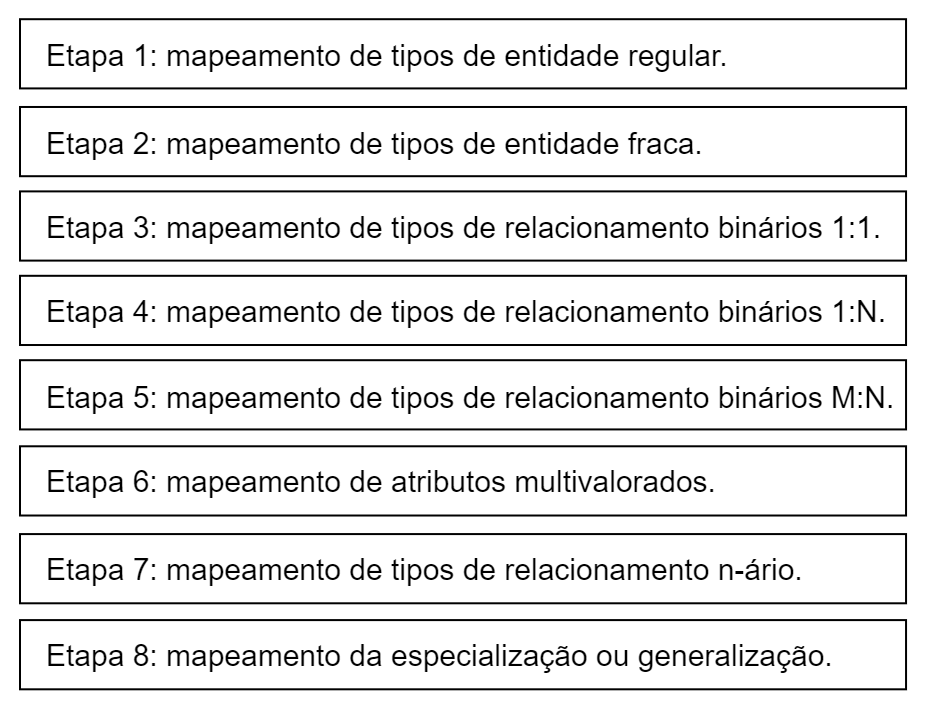
\includegraphics[scale=0.12]{Figuras/03_01.png}
\end{figure}
\end{ftst}

%==================================

\begin{ftst}{Exemplo de DER}{Mapeamento ER para relacional}
\begin{figure}
    \centering
    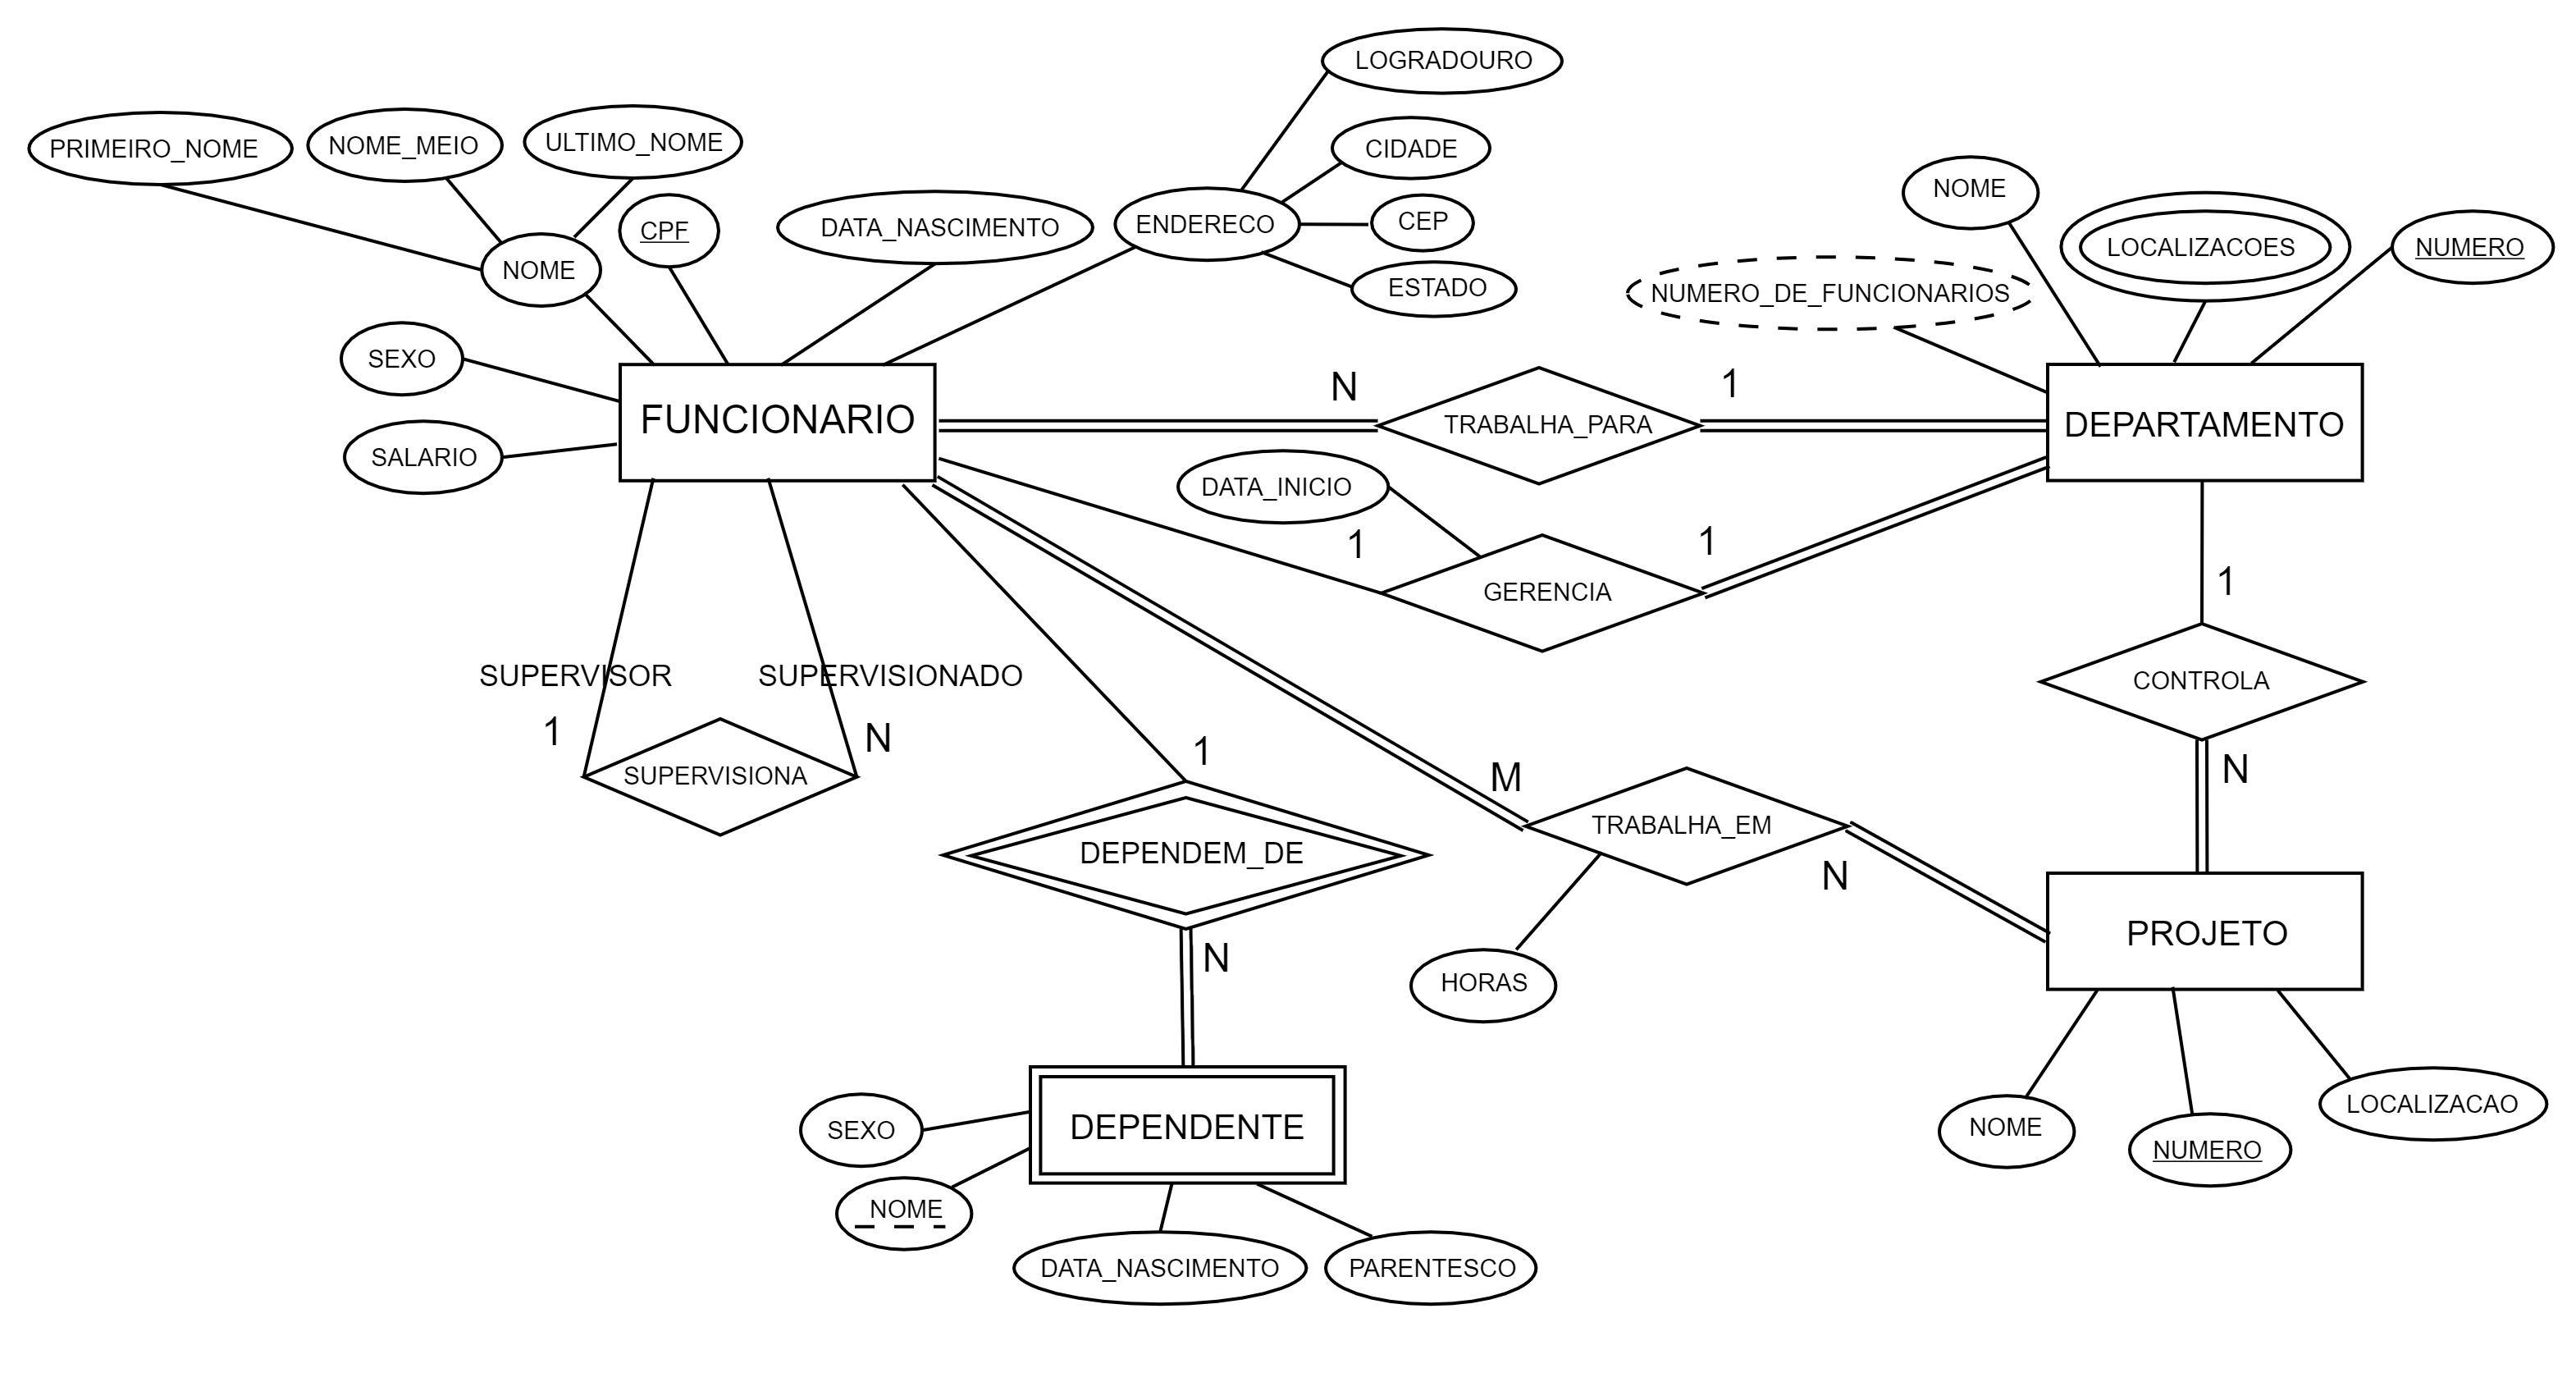
\includegraphics[scale=0.11]{Figuras/03_02.png}
\end{figure}
\end{ftst}

%==================================

\begin{ftst}{Etapa 1: entidade regular}{Mapeamento ER para relacional}
\begin{itemize}
    \item Para cada tipo de entidade regular (forte) E no esquema ER, crie uma relação R que inclua todos os atributos simples de E.
    \item Inclua apenas os atributos de componente simples de um atributo composto.
    \item Escolha um dos atributos-chave de E como chave primária para R.
    \item Se a chave escolhida de E for composta, o conjunto de atributos simples que a compõem formarão juntos a chave primária de R.
    
\end{itemize}
\end{ftst}

%==================================

\begin{ftst}{Etapa 1: entidade regular}{Mapeamento ER para relacional}
\vone
\begin{figure}
    \centering
    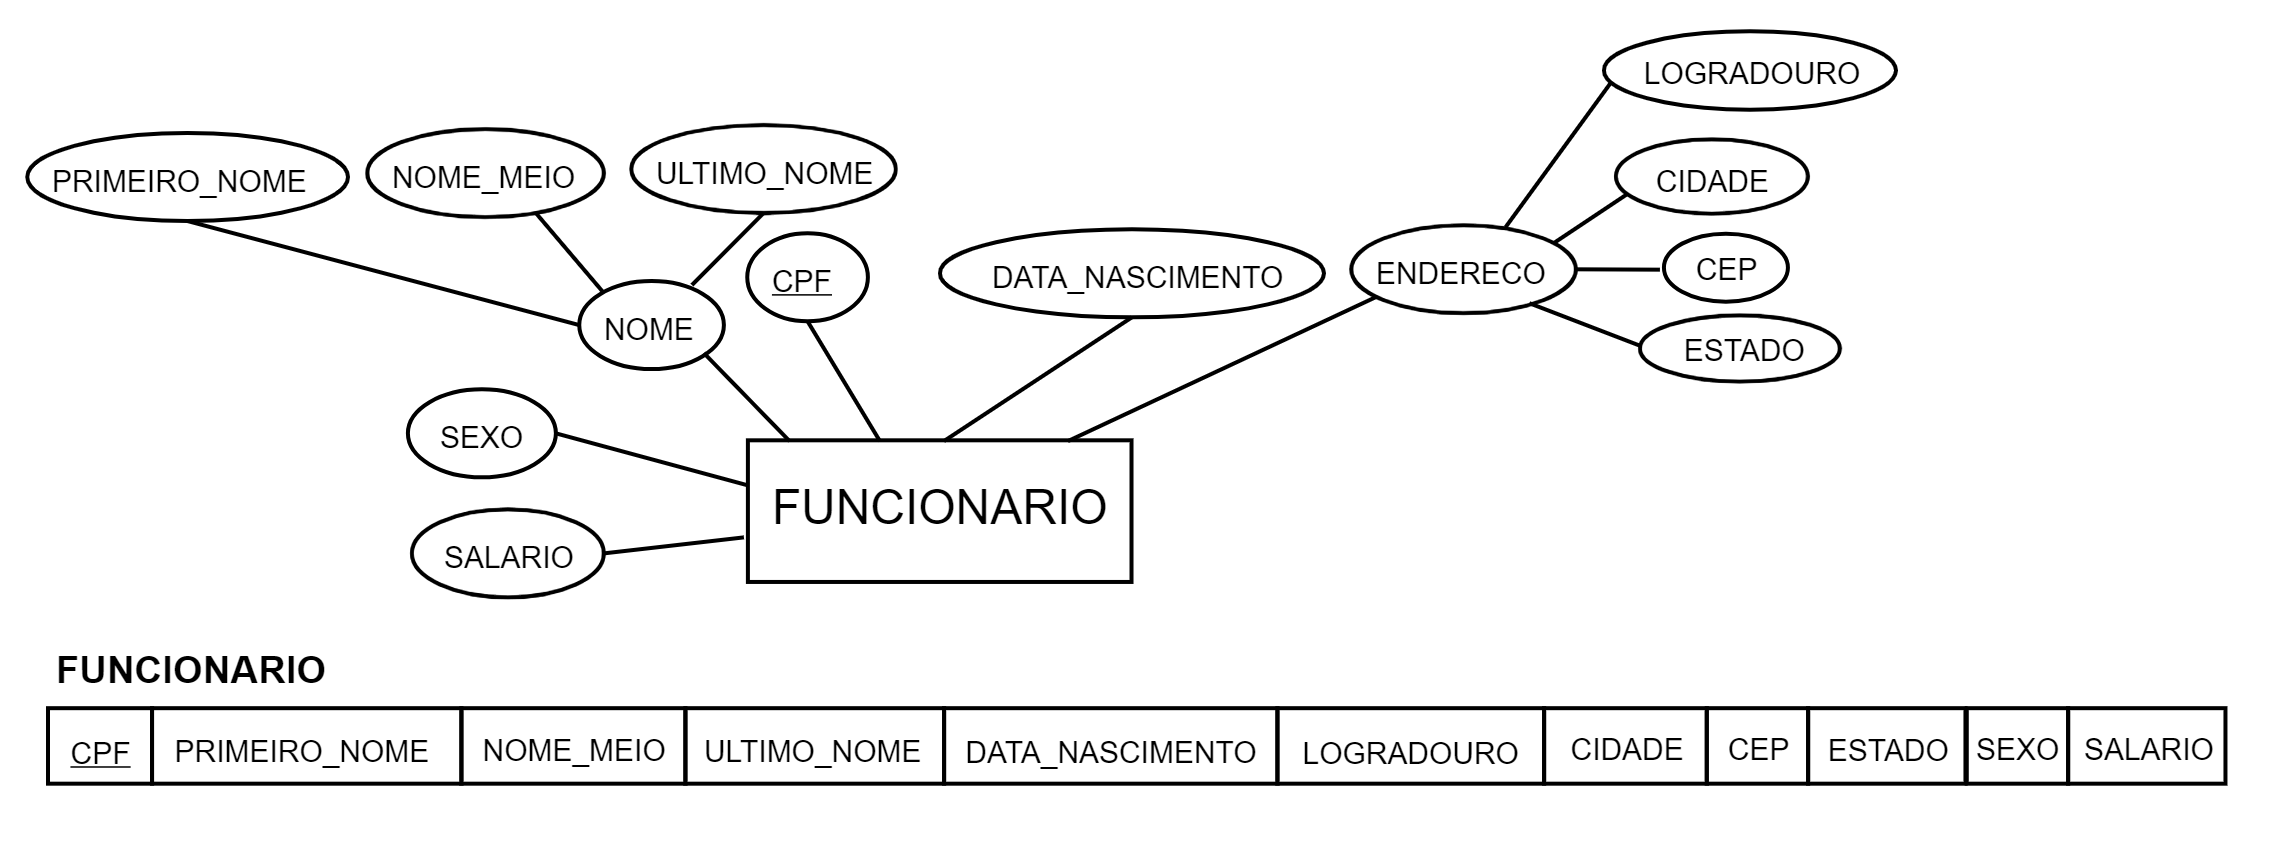
\includegraphics[scale=0.15]{Figuras/03_03.png}
\end{figure}
\end{ftst}

%==================================

\begin{ftst}{Etapa 2: entidade fraca}{Mapeamento ER para relacional}
\small
\begin{itemize}
    \item Para cada tipo de entidade fraca F no esquema ER com tipo de entidade proprietária E, crie uma relação R e inclua todos os atributos simples (ou componentes simples dos atributos compostos).
    \item inclua como atributos de chave estrangeira de R os atributos de chave primária da(s) relação(ões) que corresponde(m) aos tipos de entidade proprietária.
    \item A chave primária de R é a combinação das chaves primárias dos proprietários e a chave parcial do tipo de entidade fraca F, se houver.
    \item Se houver um tipo de entidade fraca $E_2$, cujo proprietário também é um tipo de entidade fraca $E_1$, então $E_1$ deve ser mapeado antes de $E_2$ para determinar primeiro sua chave primária.
    \item É comum escolher a opção de propagação (CASCADE) para a ação de disparo referencial na chave estrangeira na relação correspondente ao tipo de entidade fraca, pois uma entidade fraca tem uma dependência de existência em sua entidade proprietária. Isso pode ser usado para ON UPDATE e ON DELETE.
    
\end{itemize}
\end{ftst}

%==================================

\begin{ftst}{Etapa 2: entidade fraca}{Mapeamento ER para relacional}
\vone
\vone
\begin{figure}
    \centering
    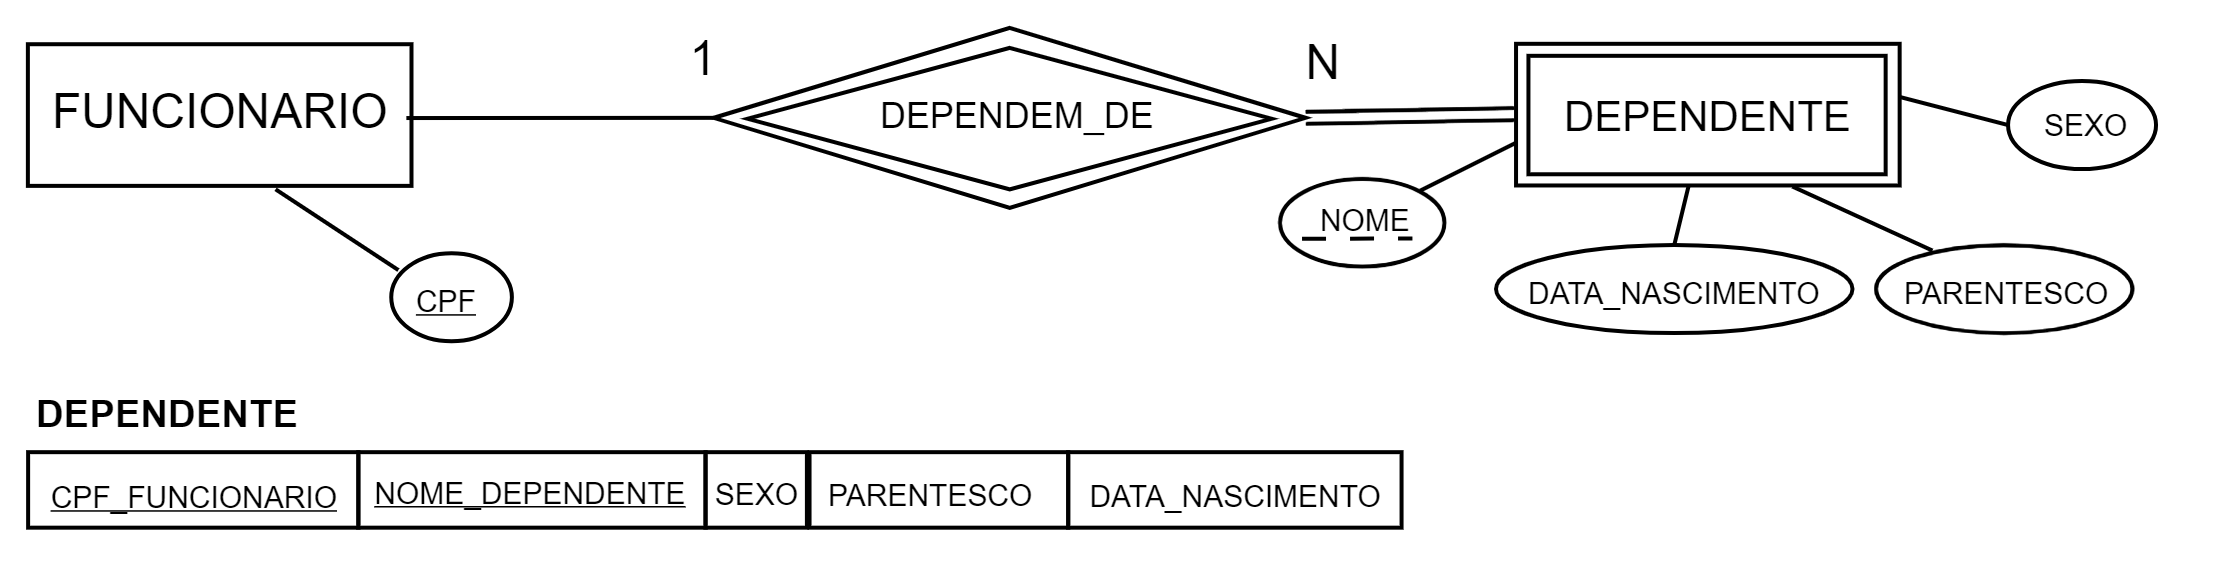
\includegraphics[scale=0.11]{Figuras/03_04.png}
\end{figure}
\end{ftst}

%==================================

\begin{ftst}{Técnicas para mapear relacionamentos}{Mapeamento ER para relacional}
A técnica da chave estrangeira:
\footnotesize
\begin{itemize}
    \item[1.]  Escolha uma entidade $S$ que participa da relação $R$ e inclua como chave estrangeira em $S$ a chave primária da outra entidade $T$. 
    \item[2.] É melhor escolher um tipo de entidade com participação total em $R$ no papel de $S$.
    \item[3.] Inclua todos os atributos simples (ou componentes simples dos atributos compostos) do relacionamento $R$ como atributos de $S$.
\end{itemize}
\begin{figure}
    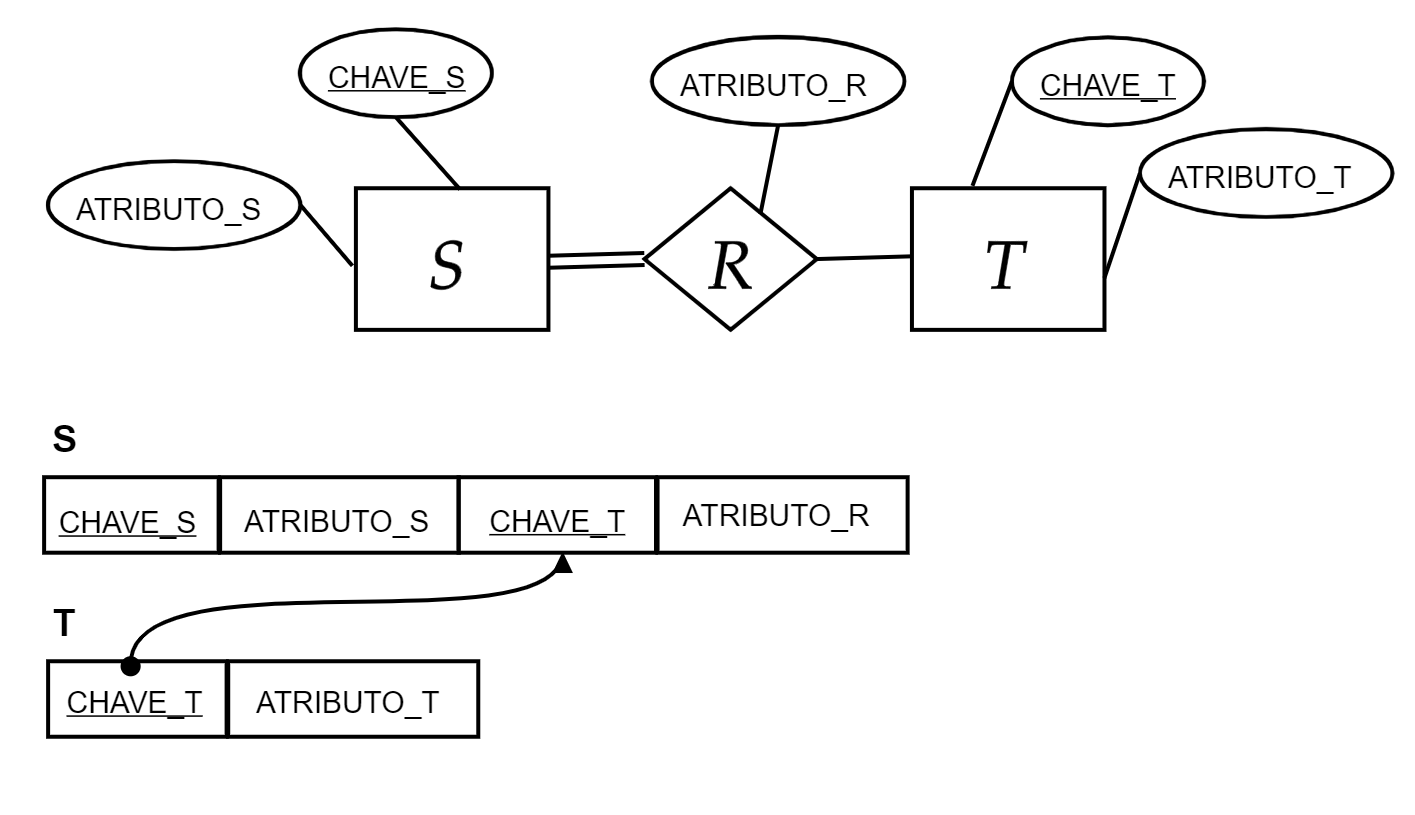
\includegraphics[scale=0.15]{Figuras/03_06.png}
\end{figure}
\end{ftst}

%==================================

\begin{ftst}{Técnicas para mapear relacionamentos}{Mapeamento ER para relacional}
A técnica de relação de referência cruzada ou relacionamento:
\footnotesize
\begin{itemize}
    \item[1.] Configurar uma terceira relação $R$ para a finalidade de referência cruzada das chaves primárias das duas relações $S$ e $T$.
    \item[2.] Inclua como atributos de chave estrangeira em $R$ as chaves primárias das relações que representam as entidades participantes.
    \item[3.] Defina como chave primária de $R$, a combinação das suas chaves estrangeiras.
    \item[4.] Inclua também quaisquer atributos simples do relacionamento.

\end{itemize}
\begin{figure}
    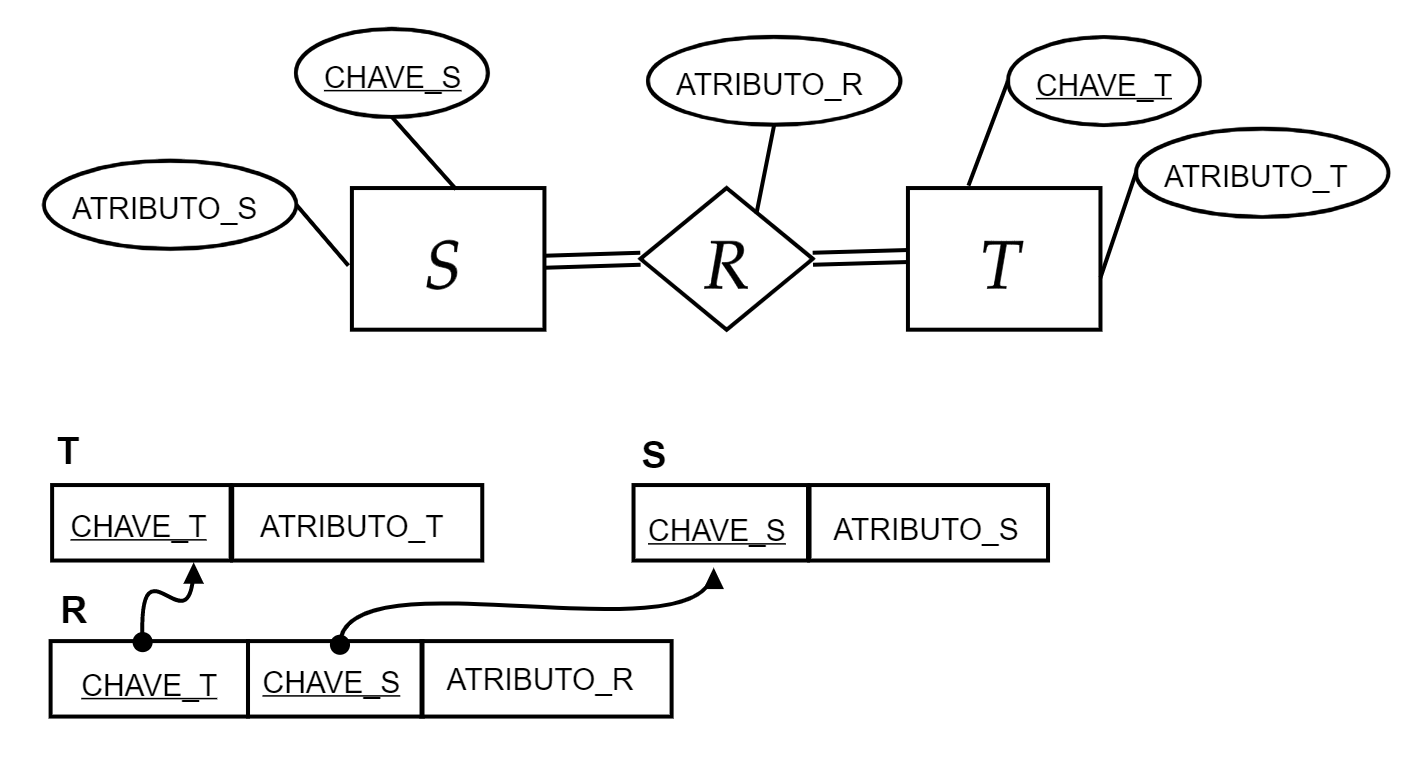
\includegraphics[scale=0.15]{Figuras/03_07.png}
\end{figure}
\end{ftst}

%==================================

\begin{ftst}{Técnicas para mapear relacionamentos}{Mapeamento ER para relacional}
A técnica de relação combinada:
\footnotesize
\begin{itemize}
    \item[1.] Combinar as duas entidades e o relacionamento em uma única relação $R$.
\end{itemize}
\begin{figure}
    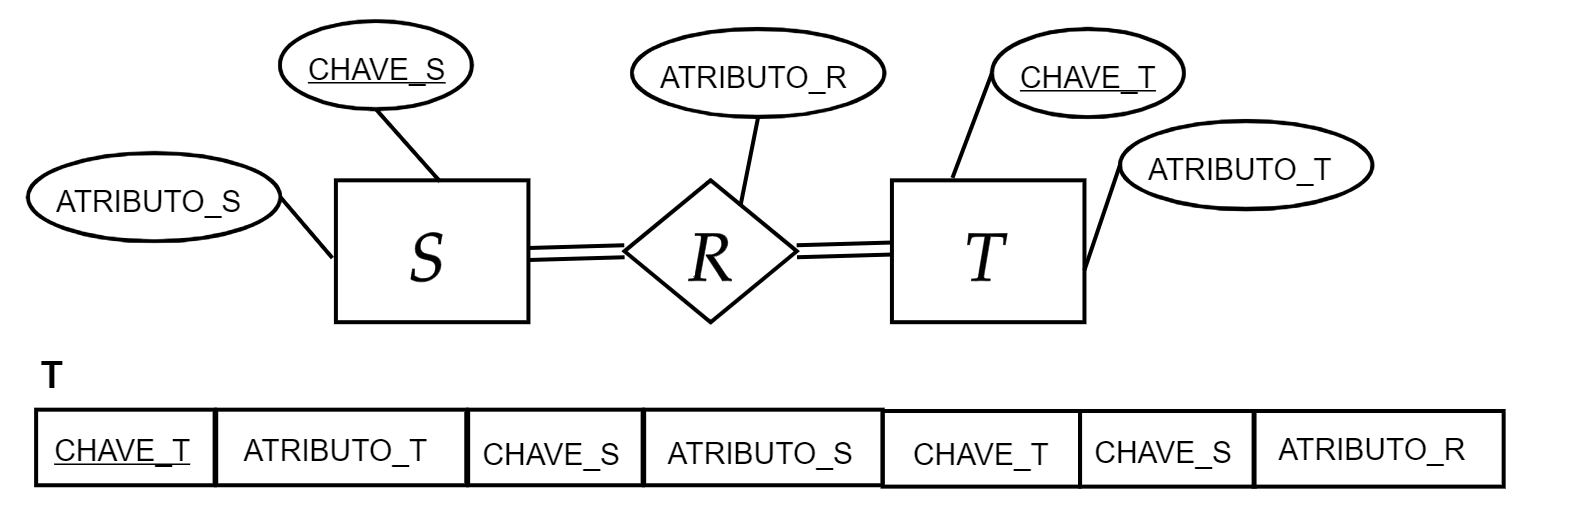
\includegraphics[scale=0.17]{Figuras/03_08.png}
\end{figure}
\end{ftst}

%==================================

\begin{ftst}{Etapa 3: relacionamento binário 1:1}{Mapeamento ER para relacional}
\begin{itemize}
    \item É possível usar as 3 técnicas, mas a técnica de chave estrangeira é a mais útil e deve ser seguida, a menos que haja condições especiais.
\end{itemize}

\begin{figure}
    \centering
    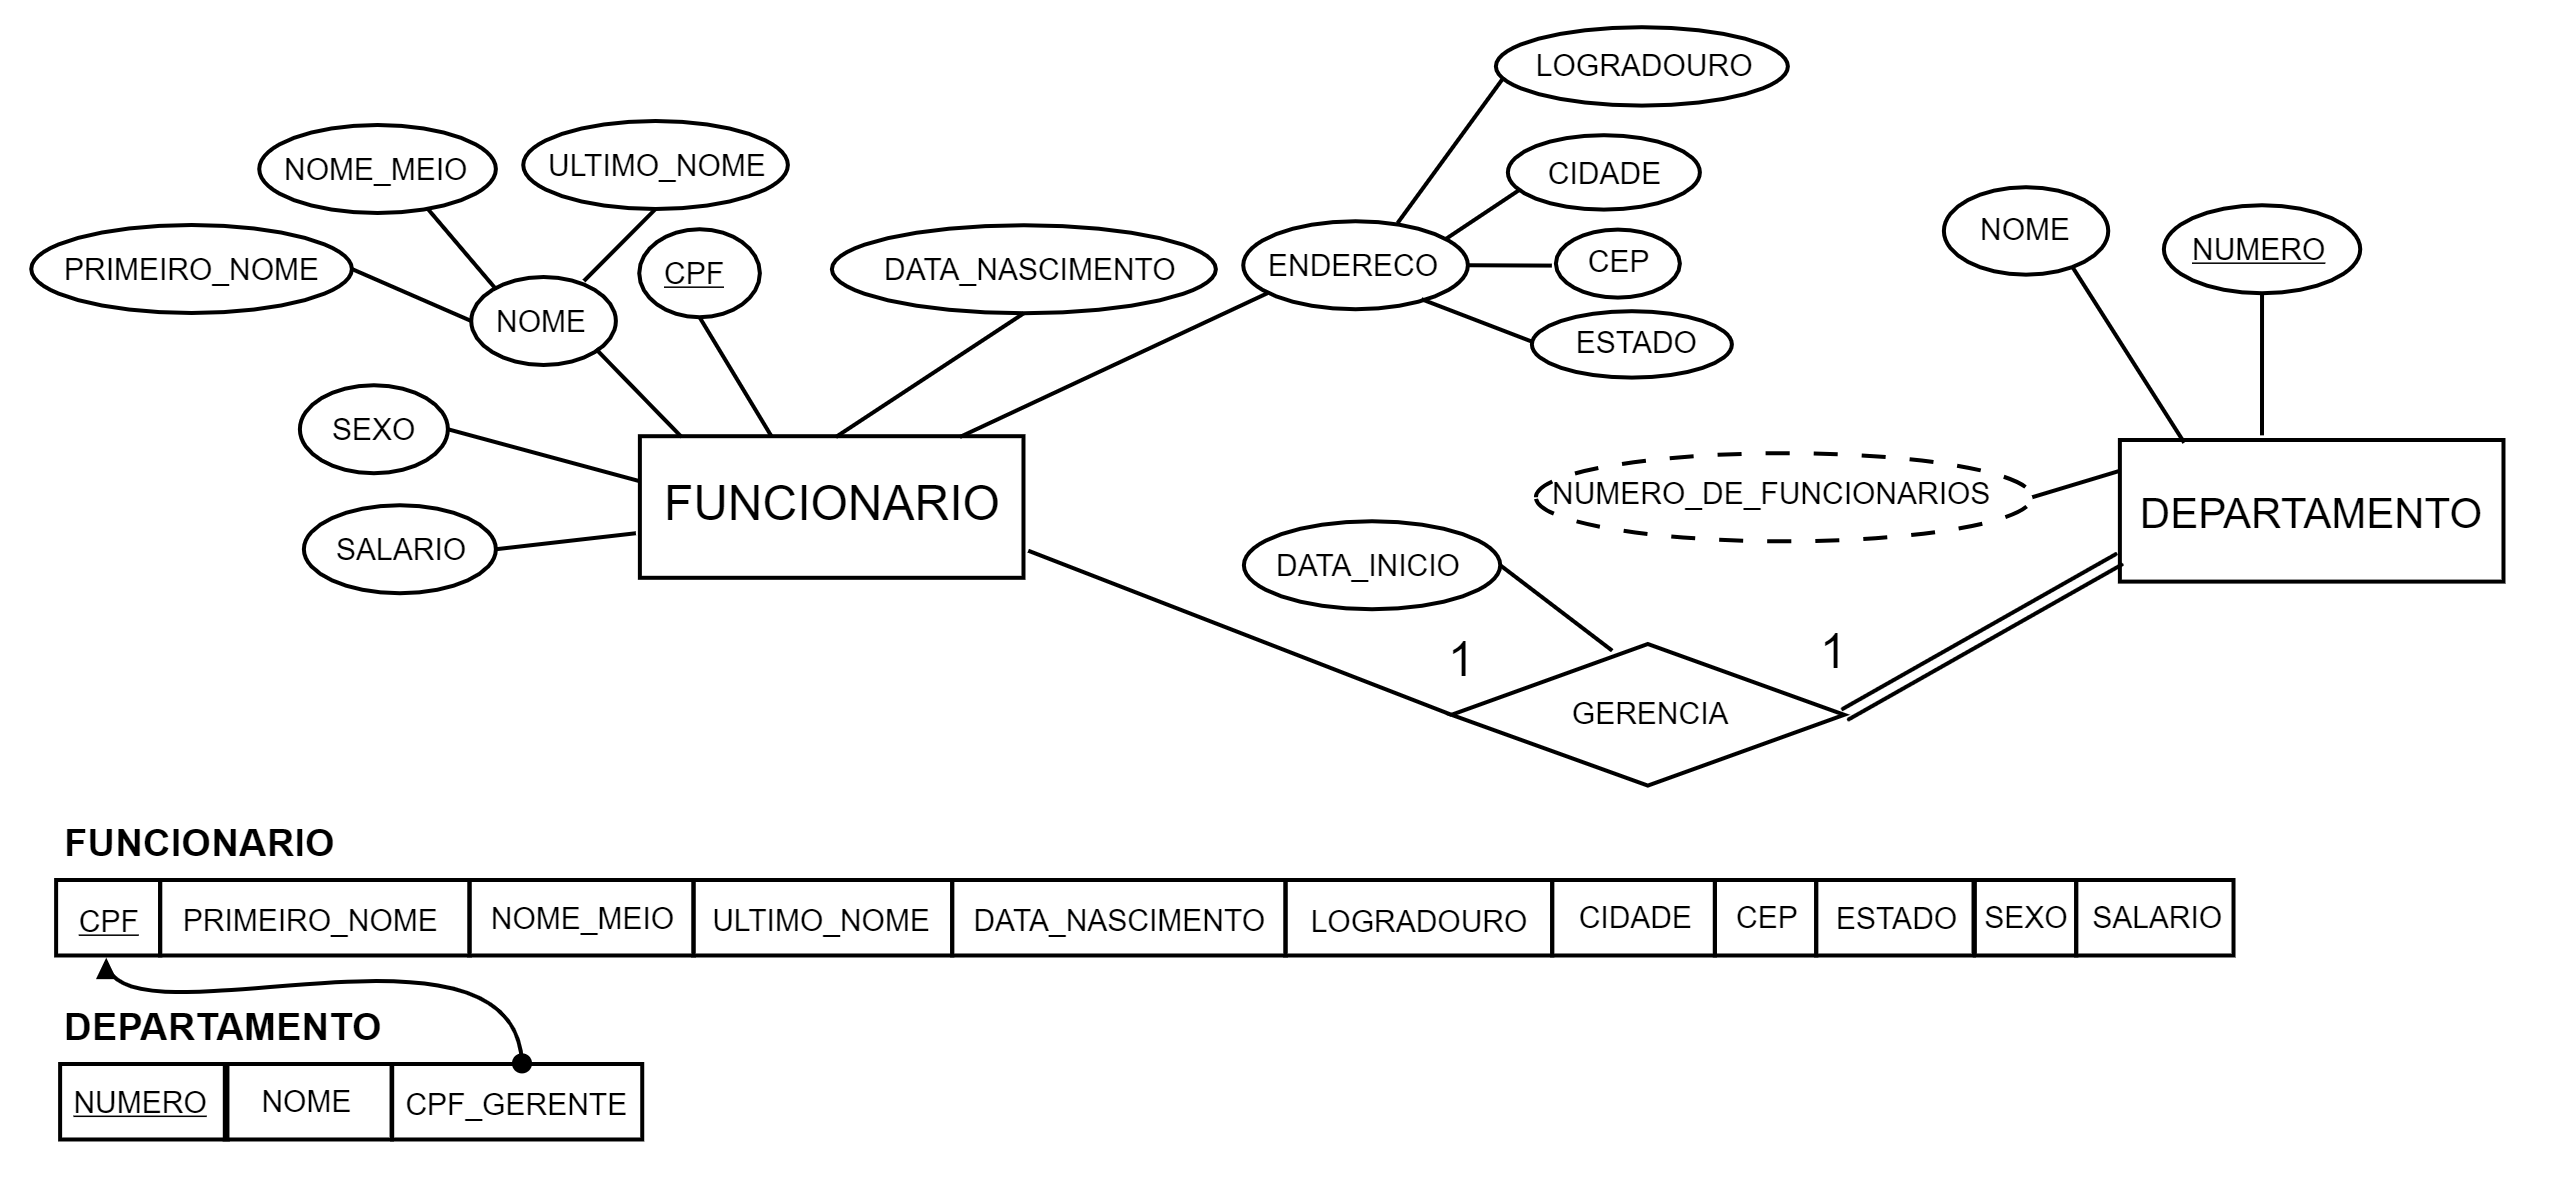
\includegraphics[scale=0.12]{Figuras/03_05.png}
\end{figure}
\end{ftst}

%==================================

\begin{ftst}{Etapa 4: relacionamento binário 1:N}{Mapeamento ER para relacional}
\small
\begin{itemize}
    \item Existem duas técnicas possíveis: a técnica de chave estrangeira e a técnica de relação de referência cruzada ou relacionamento. 
    \item A primeira geralmente é a preferida, pois reduz o número de tabelas.
\end{itemize}
\begin{figure}
    \centering
    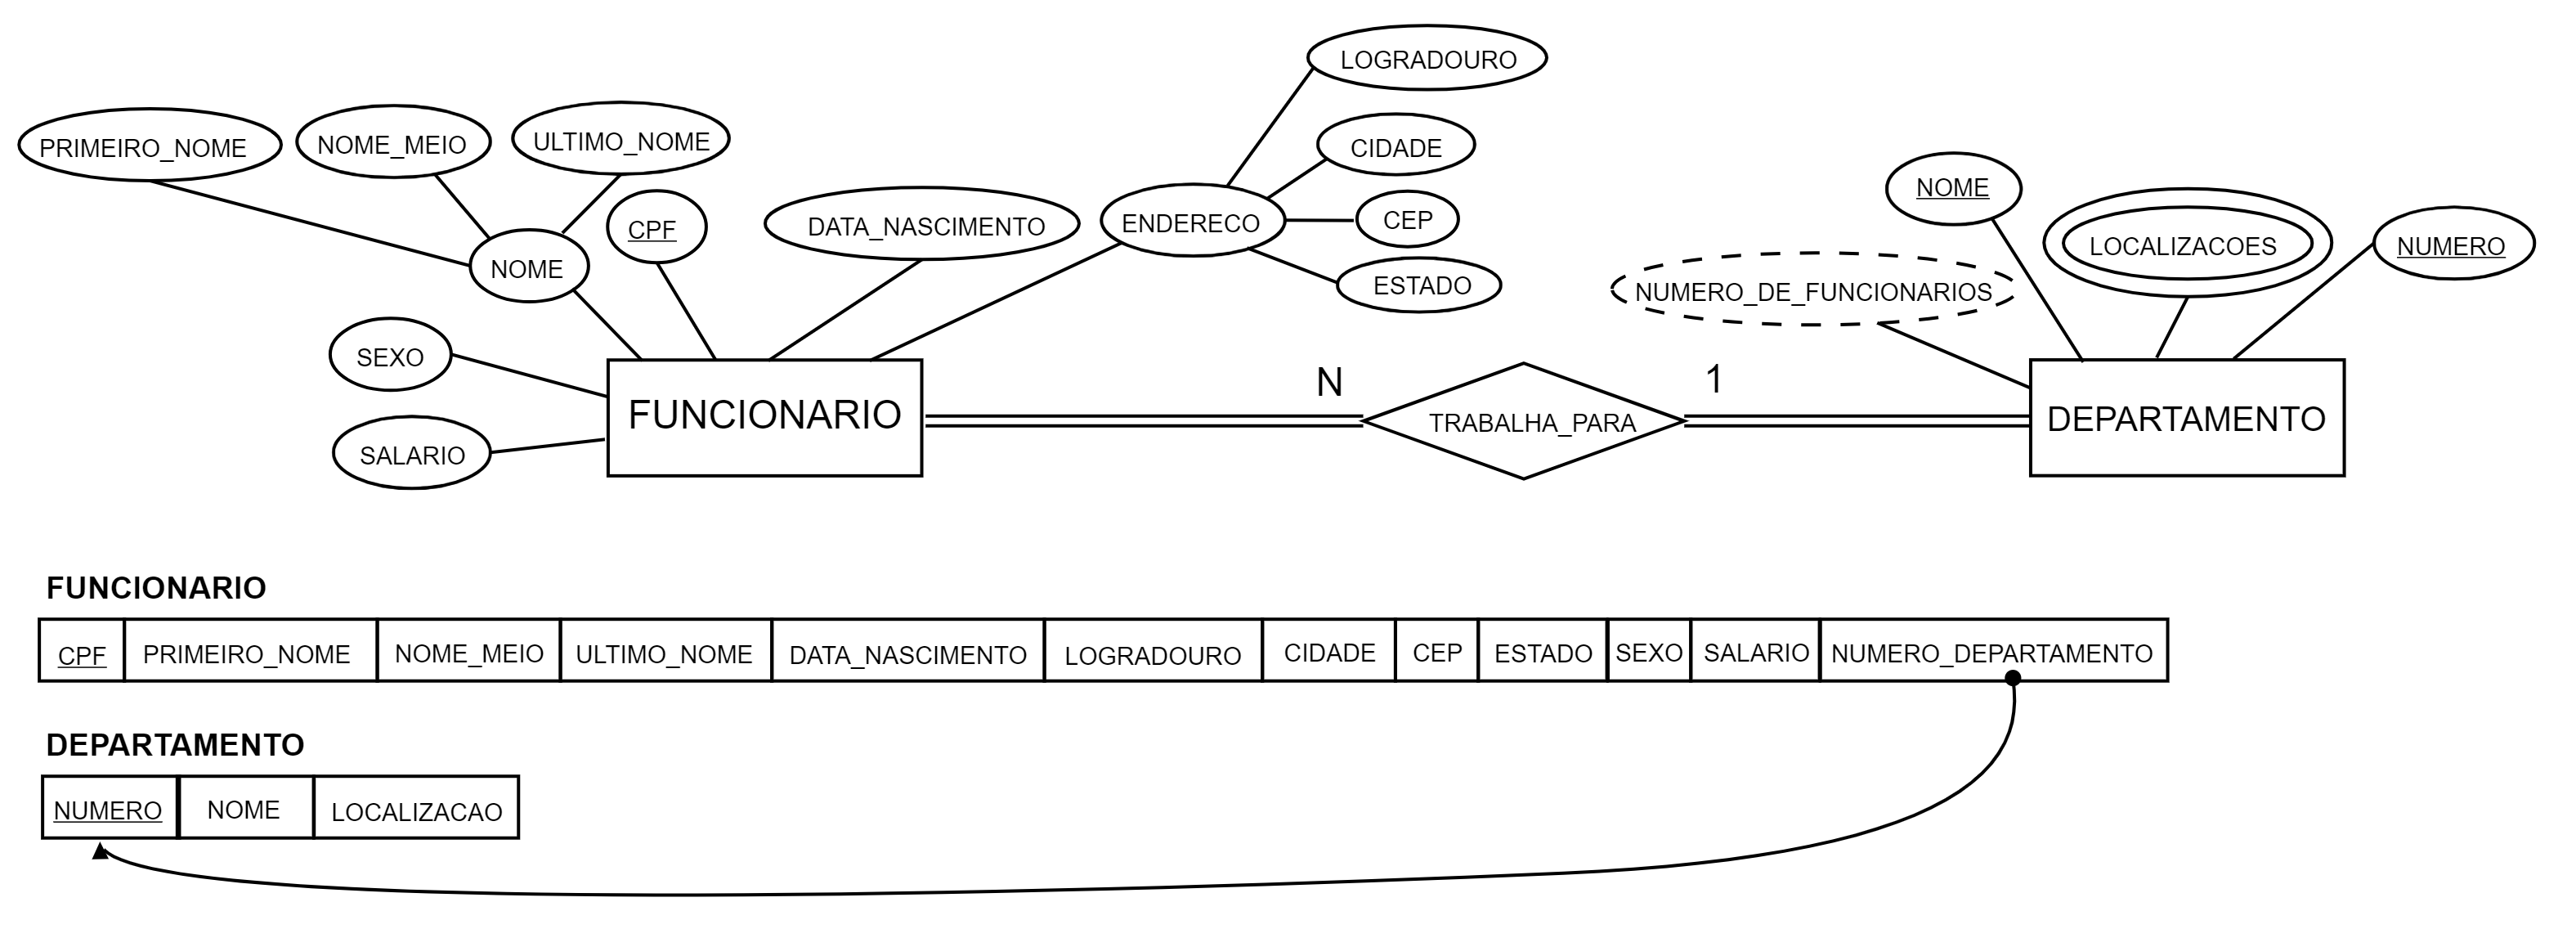
\includegraphics[scale=0.11]{Figuras/03_09.png}
\end{figure}
\end{ftst}

%==================================

\begin{ftst}{Etapa 5: relacionamento binário M:N}{Mapeamento ER para relacional}
\small
\begin{itemize}
    \item A única operação para relacionamentos M:N é a opção de relação de relacionamento.
\end{itemize}
\begin{figure}
    \centering
    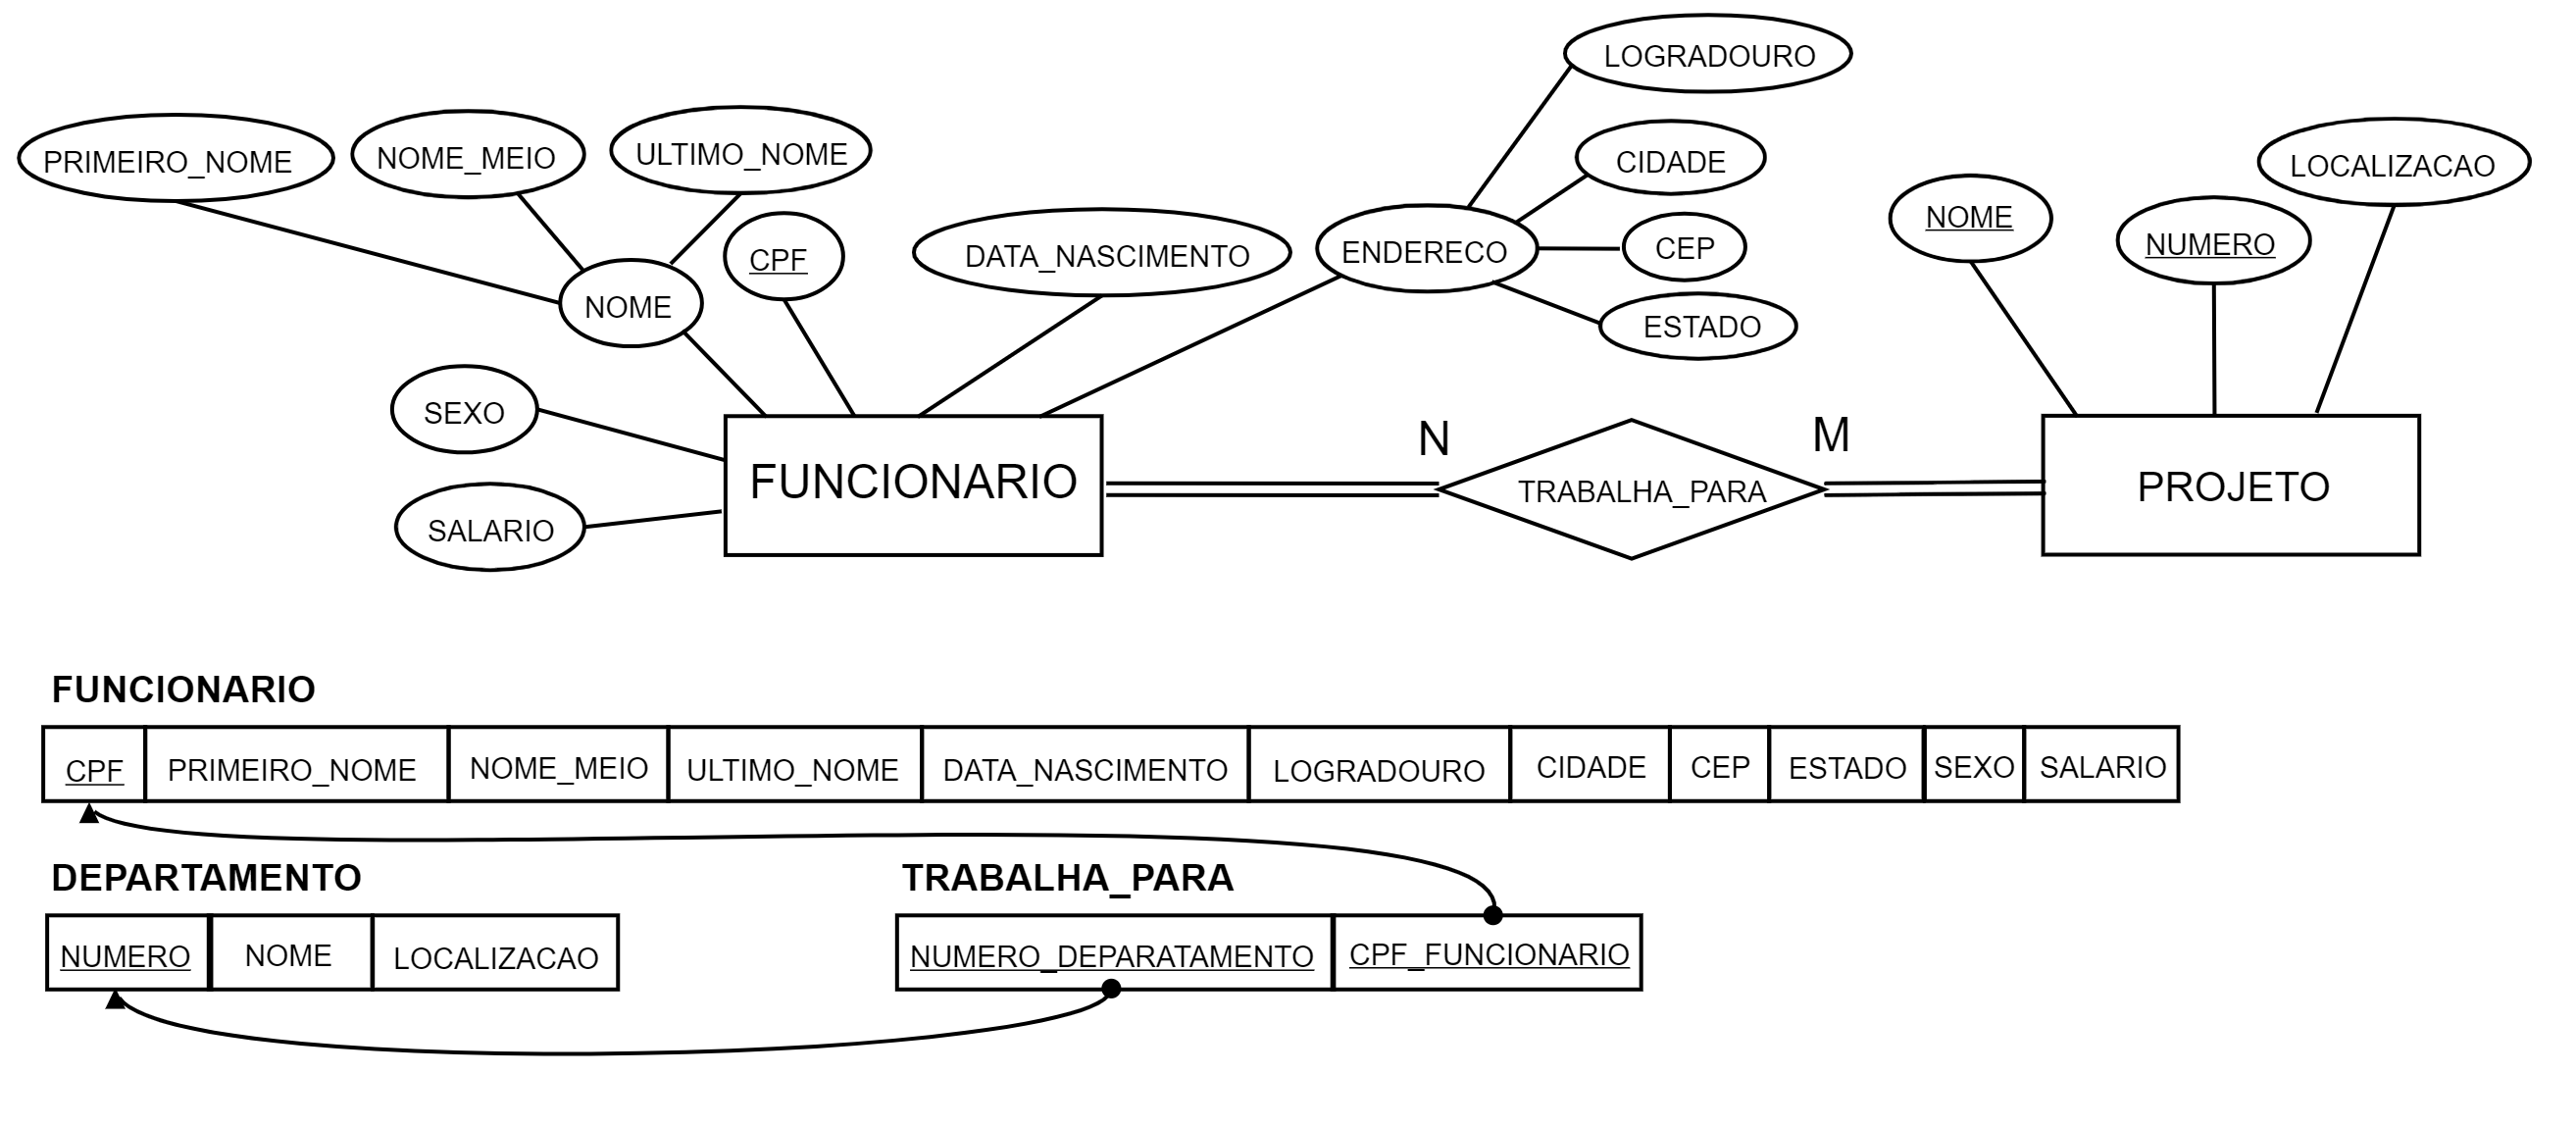
\includegraphics[scale=0.12]{Figuras/03_10.png}
\end{figure}
\end{ftst}

%==================================

\begin{ftst}{Etapa 6: mapeamento de atributos multivalorados}{Mapeamento ER para relacional}
\begin{itemize}
    \item Para cada atributo multivalorado $A$, crie uma nova relação $R$.
    \item Essa relação $R$ incluirá um atributo correspondente a $A$, mais o atributo da chave primária $Ch$ de $A$ como chave estrangeira.
    \item A chave primária de $R$ é a combinação de $A$ e $Ch$.
    \item Se o atributo multivalorado for composto, incluímos seus componentes simples.
\end{itemize}
\begin{figure}
    \centering
    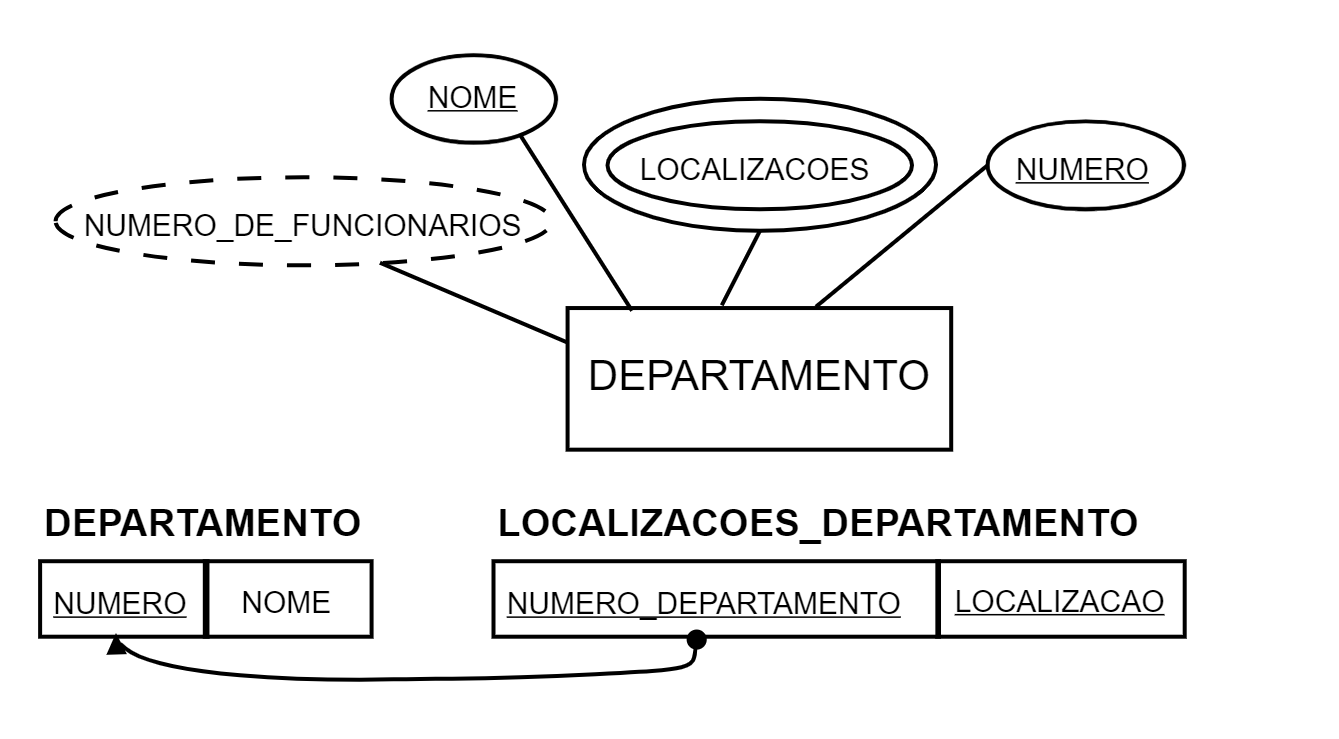
\includegraphics[scale=0.15]{Figuras/03_11.png}
\end{figure}

\end{ftst}

%==================================

\begin{ftst}{Etapa 7: mapeamento de relacionamento n-ário}{Mapeamento ER para relacional}
\small
\begin{itemize}
    \item Usamos a opção de relação de relacionamento.
    \item Para cada tipo de relacionamento n-ário $R$, em que $n > 2$, crie uma nova relação $S$ para representar $R$.
\end{itemize}
\begin{figure}
    \centering
    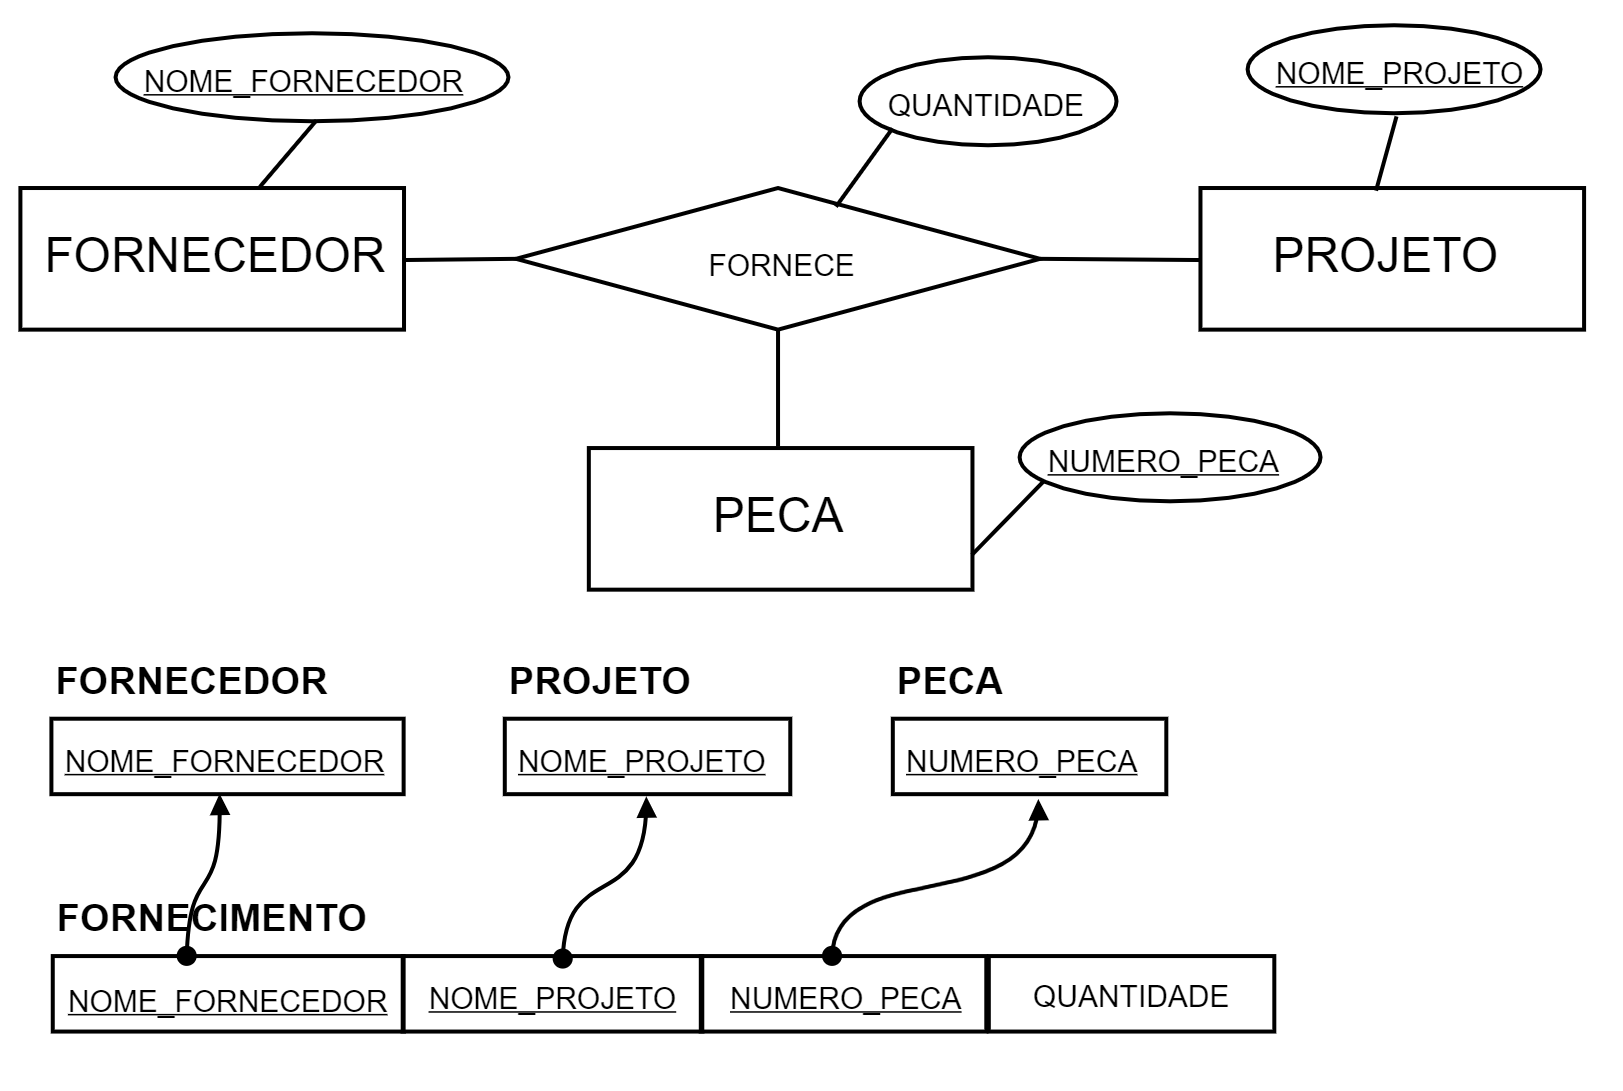
\includegraphics[scale=0.15]{Figuras/03_12.png}
\end{figure}
\end{ftst}

%==================================

\begin{ftst}{Etapa 8: mapeamento da especialização ou generalização}{Mapeamento ER para relacional}
\small
São 4 opções:
\begin{itemize}
    \item Opção 1: uma única tabela para a Hierarquia com um atributo de tipo.
    \item Opção 2: uma única tabela para a Hierarquia com múltiplos atributos booleanos.
    \item Opção 3: uma tabela para cada subclasse com tabela para a superclasse. 
    \item Opção 4: uma tabela para cada subclasse sem tabela para a superclasse. 
\end{itemize}
\end{ftst}

%==================================

\begin{ftst}{Etapa 8: mapeamento da especialização ou generalização}{Mapeamento ER para relacional}
\small
Para a opção 1: tabela única.
\begin{itemize}
    \item Inserir na tabela um atributo cujo valor discrimina a subclasse.
    \item Unir todos os atributos numa única tabela pode produzir valores nulos. 
    \item Usada para classes disjuntas.
\end{itemize}
\begin{figure}
    \centering
    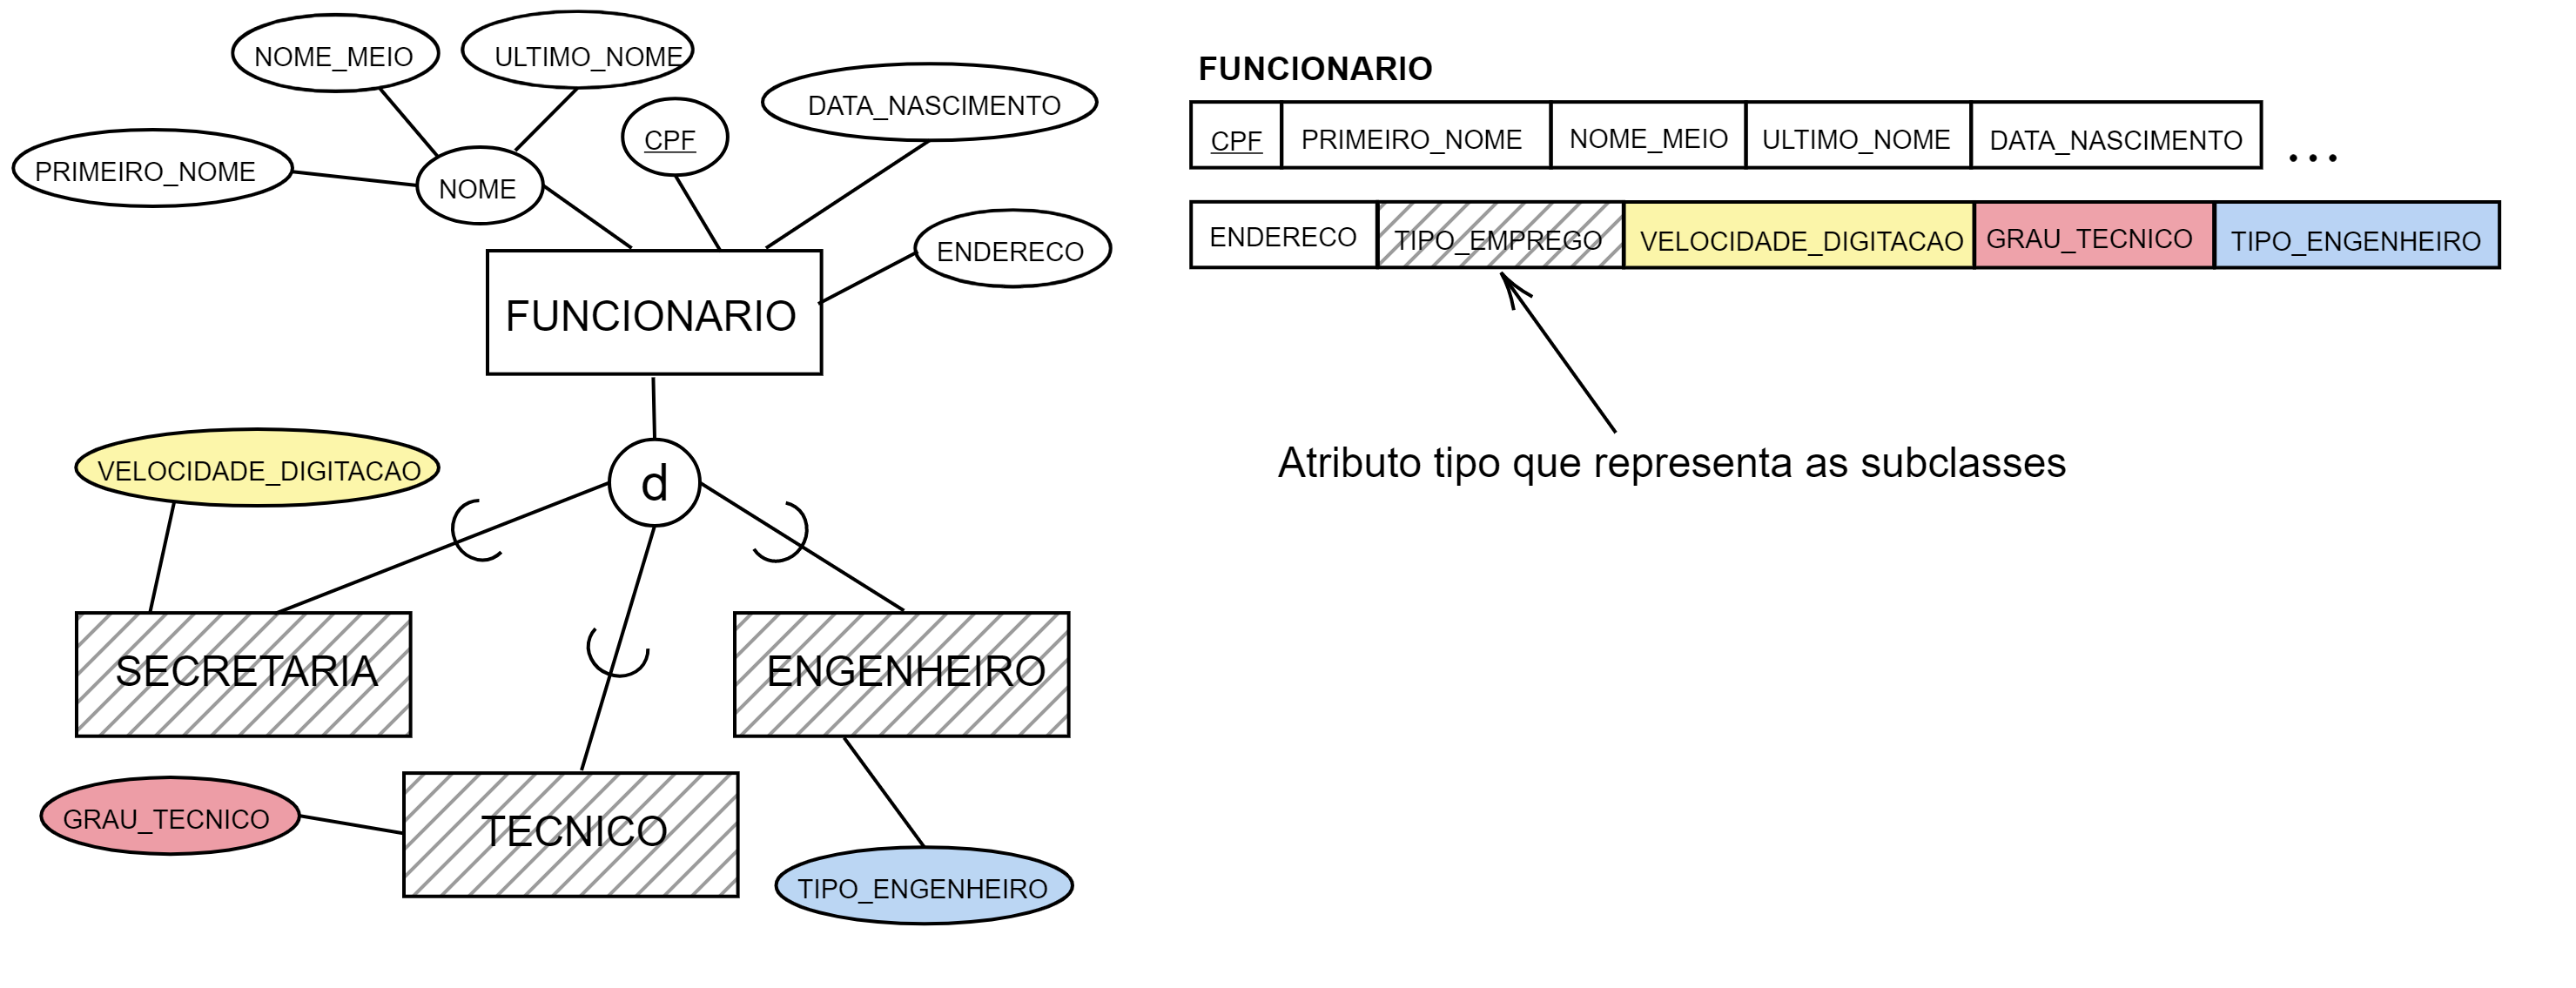
\includegraphics[scale=0.11]{Figuras/03_13.png}
\end{figure}
\end{ftst}

%==================================

\begin{ftst}{Etapa 8: mapeamento da especialização ou generalização}{Mapeamento ER para relacional}
\small
Para a opção 2: tabela única.
\begin{itemize}
    \item Inserir na tabela um atributo booleano para cada tipo de subclasse.
    \item Unir todos os atributos numa única tabela pode produzir valores nulos. 
    \item Usada para classes não disjuntas.
\end{itemize}
\begin{figure}
    \centering
    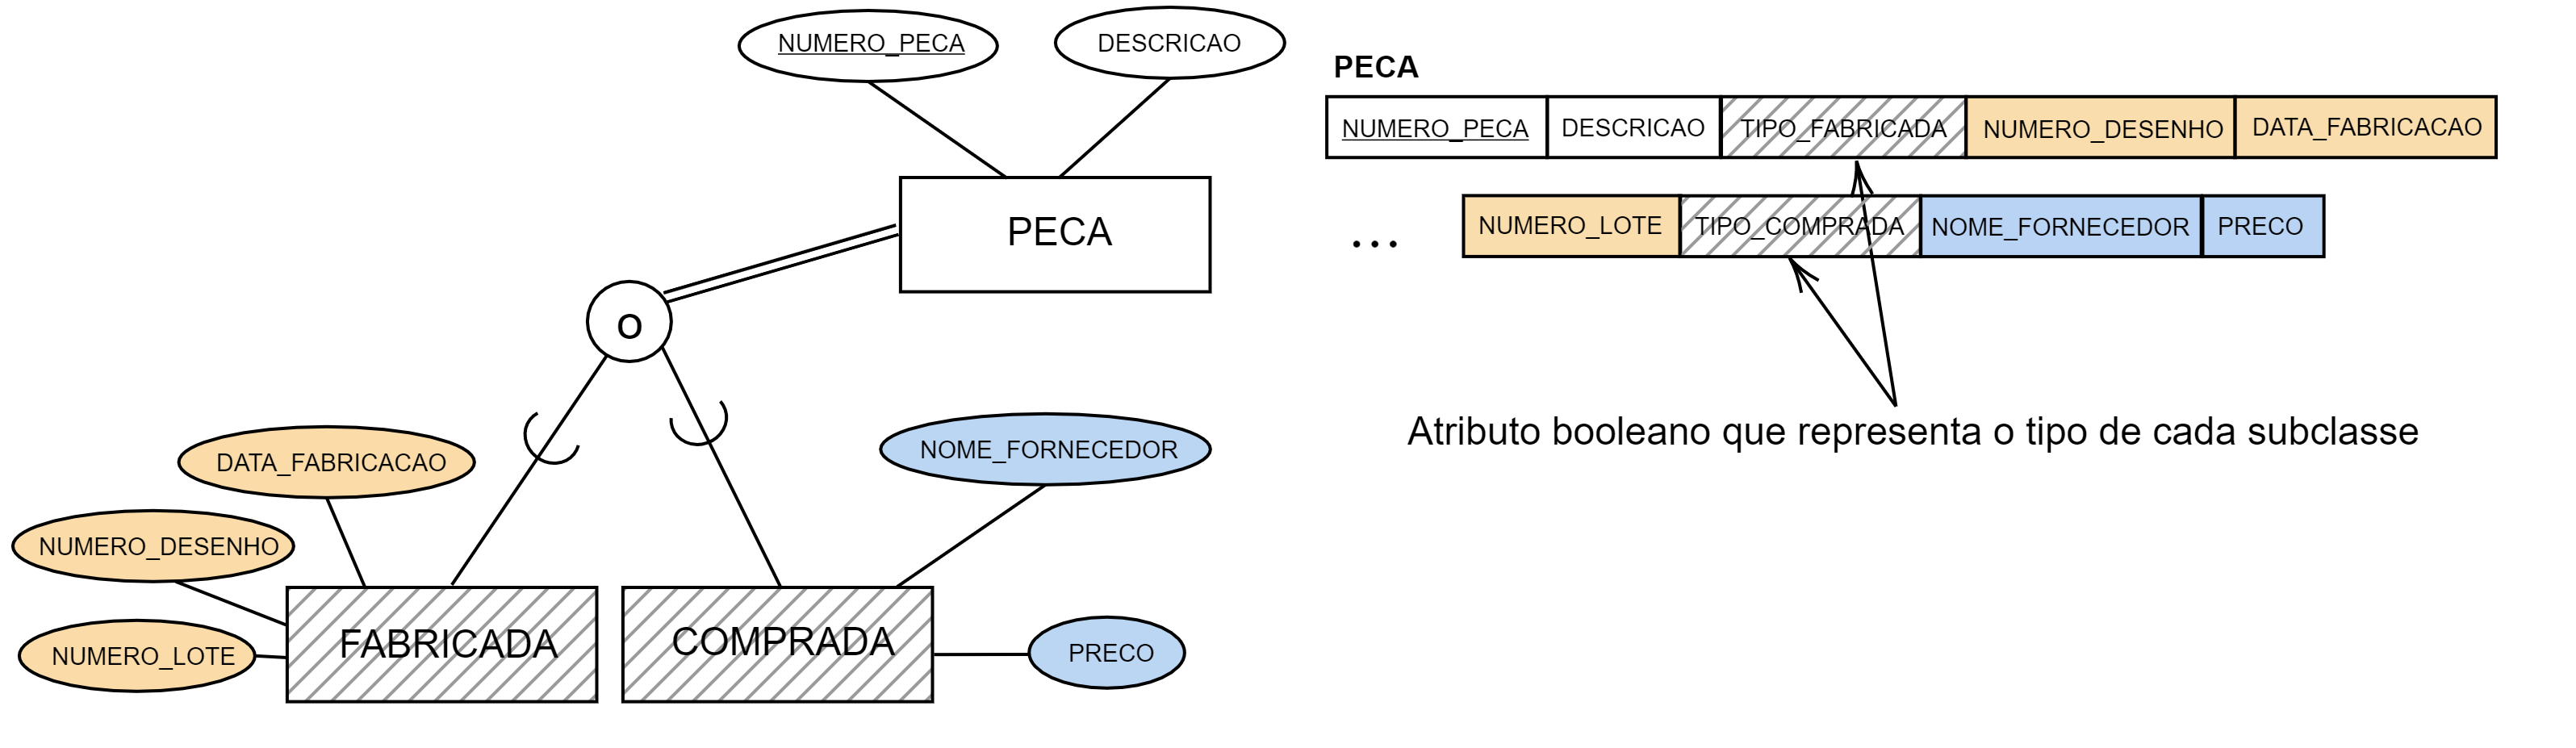
\includegraphics[scale=0.11]{Figuras/03_14.png}
\end{figure}
\end{ftst}

%==================================

\begin{ftst}{Etapa 8: mapeamento da especialização ou generalização}{Mapeamento ER para relacional}
\small
Para a opção 3: uma tabela para cada subclasse e superclasse.
\begin{itemize}
    \item A tabela da superclasse contém os atributos comuns + chave primária $ch$.
    \item Cada subclasse gera uma tabela própria com seus atributos específicos + chave primária $ch$, que também é estrangeira. 
\end{itemize}
\begin{figure}
    \centering
    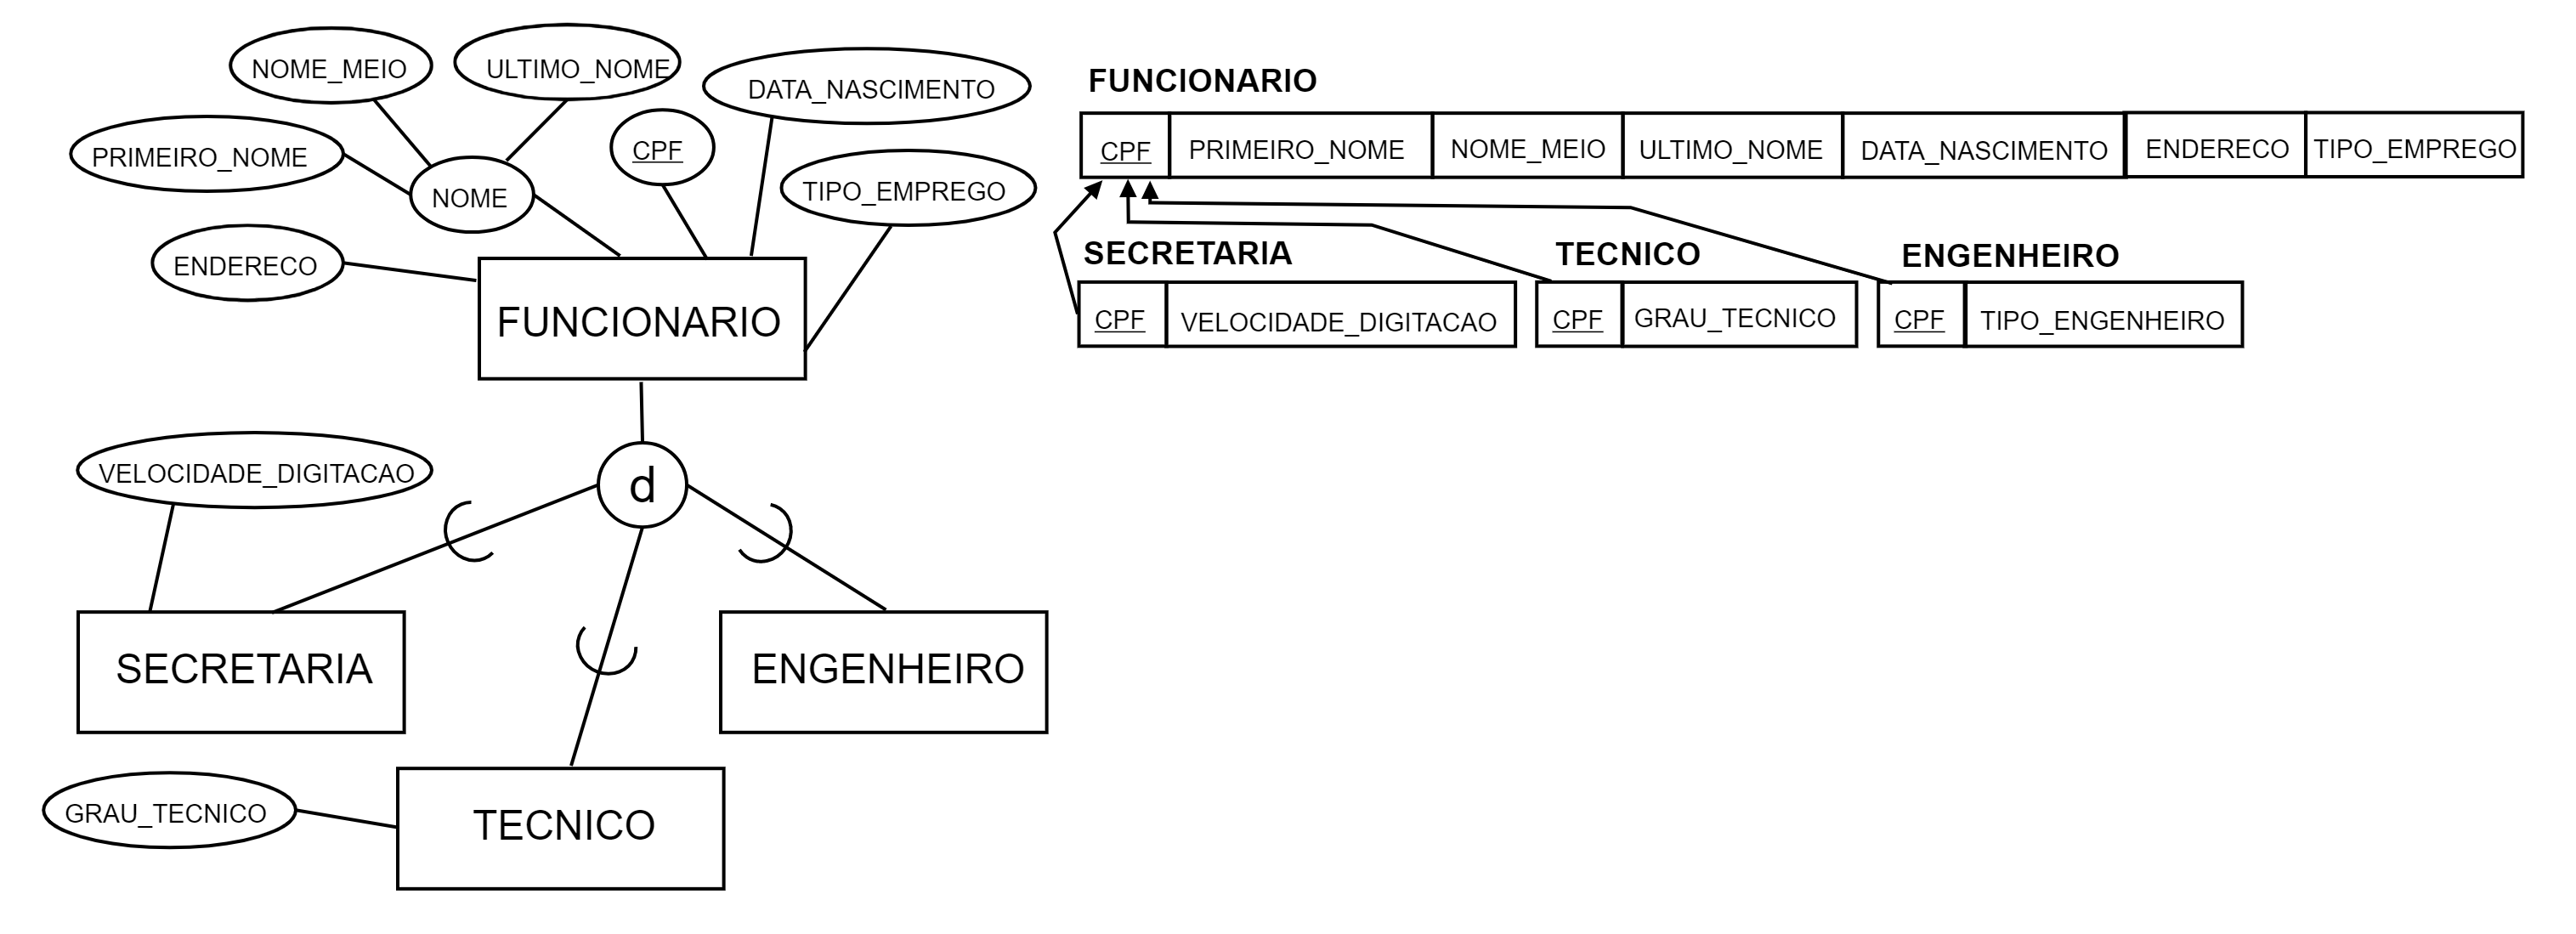
\includegraphics[scale=0.11]{Figuras/03_15.png}
\end{figure}
\end{ftst}

%==================================

\begin{ftst}{Etapa 8: mapeamento da especialização ou generalização}{Mapeamento ER para relacional}
\small
Para a opção 4: uma tabela para cada subclasse.
\begin{itemize}
    \item Cada subclasse gera uma tabela própria com seus atributos específicos + atributos da superclasse.
    \item Usada somente para especializações totais.
    \item Em caso de uso em subclasses não disjuntas, os atributos são duplicados e podem causar inconsistências.
\end{itemize}
\begin{figure}
    \centering
    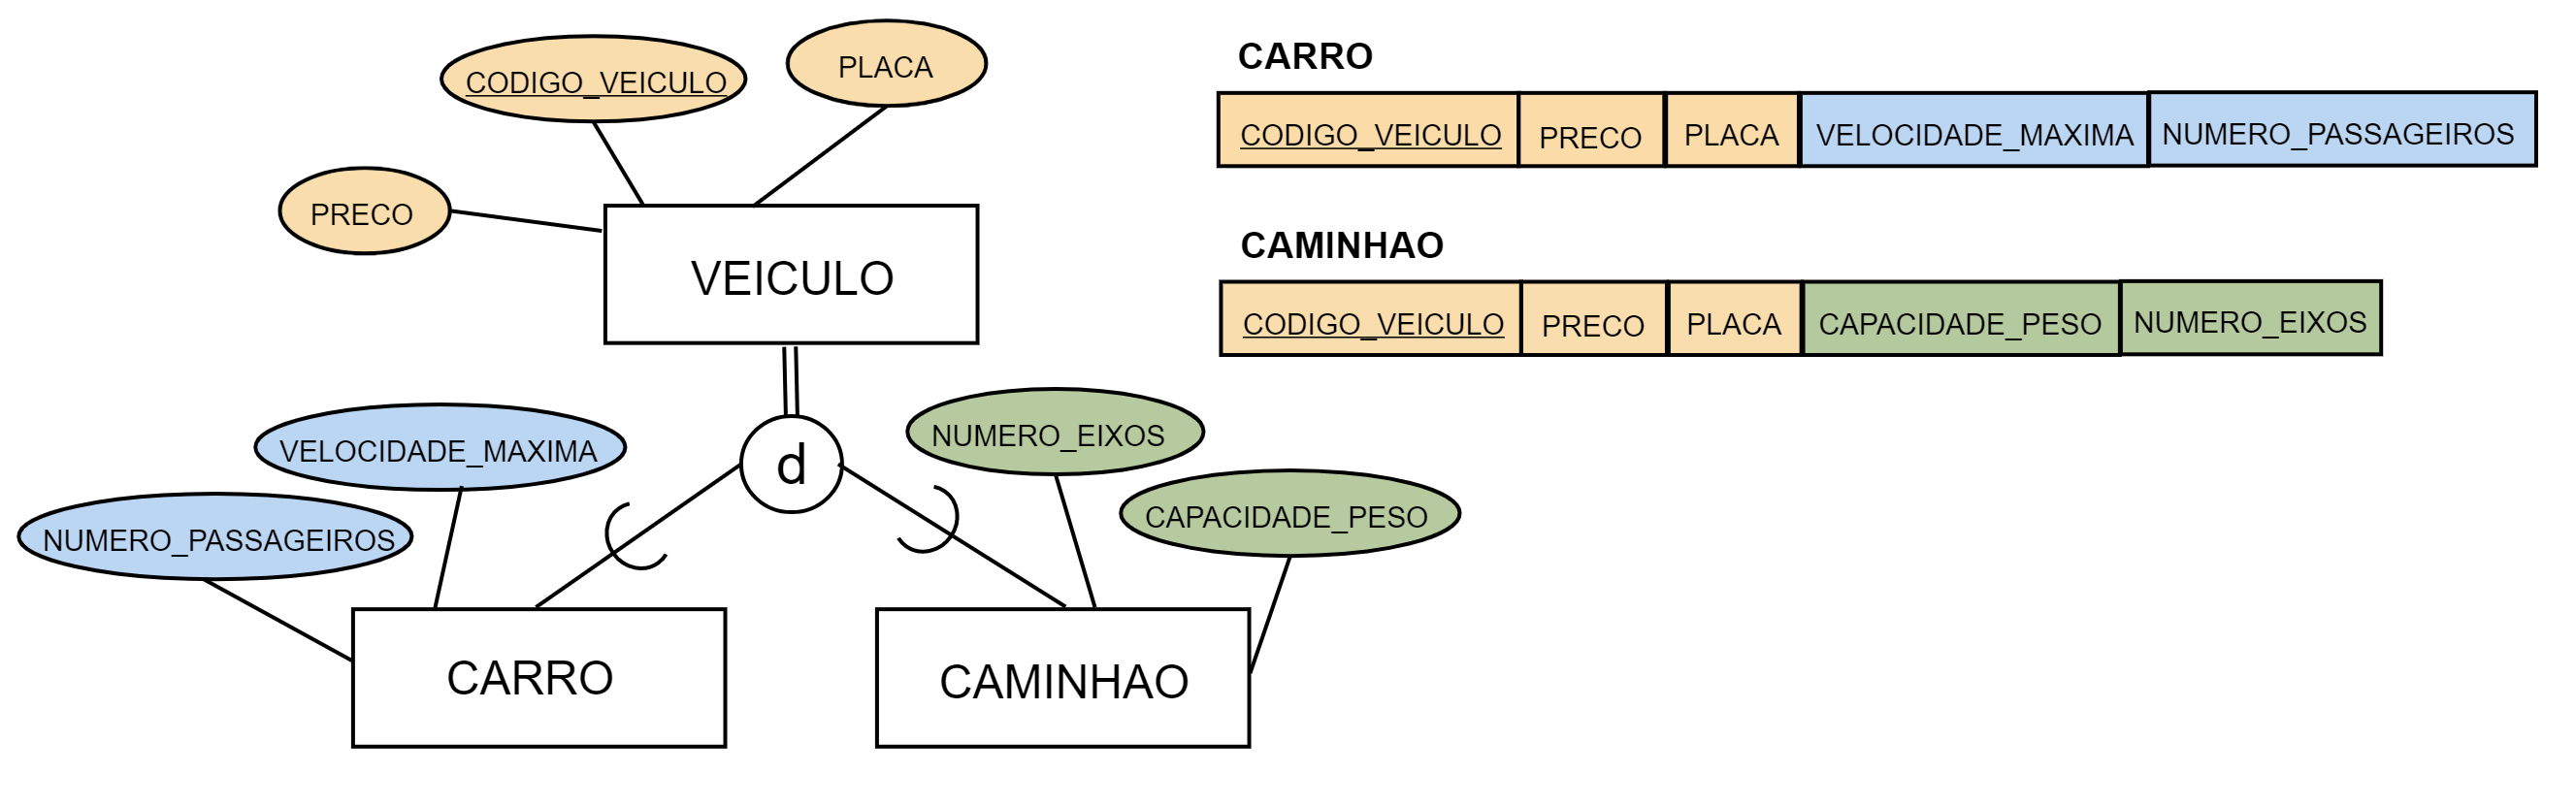
\includegraphics[scale=0.11]{Figuras/03_16.png}
\end{figure}
\end{ftst}

%==================================

\begin{ftst}{Mapeamento de subclasses compartilhadas (herança múltipla)}{Mapeamento ER para relacional}
\small
Pode ser usada qualquer uma das opções apresentadas na Etapa 8.


\end{ftst}

%==================================

\begin{ftst}{Etapa 9: mapeamento de categorias (tipos de união)}{Mapeamento ER para relacional}
\small
\begin{itemize}
    \item Crie uma tabela para a entidade que representa a união.
    \item Quando as chaves das superclasses são diferentes, cria-se um novo atributo-chave (chave substituta) para a nova tabela que corresponde a união.
    \item Para uma categoria cujas superclasses têm a mesma chave, não há necessidade de uma chave substituta.
\end{itemize}

\begin{figure}
    \centering
    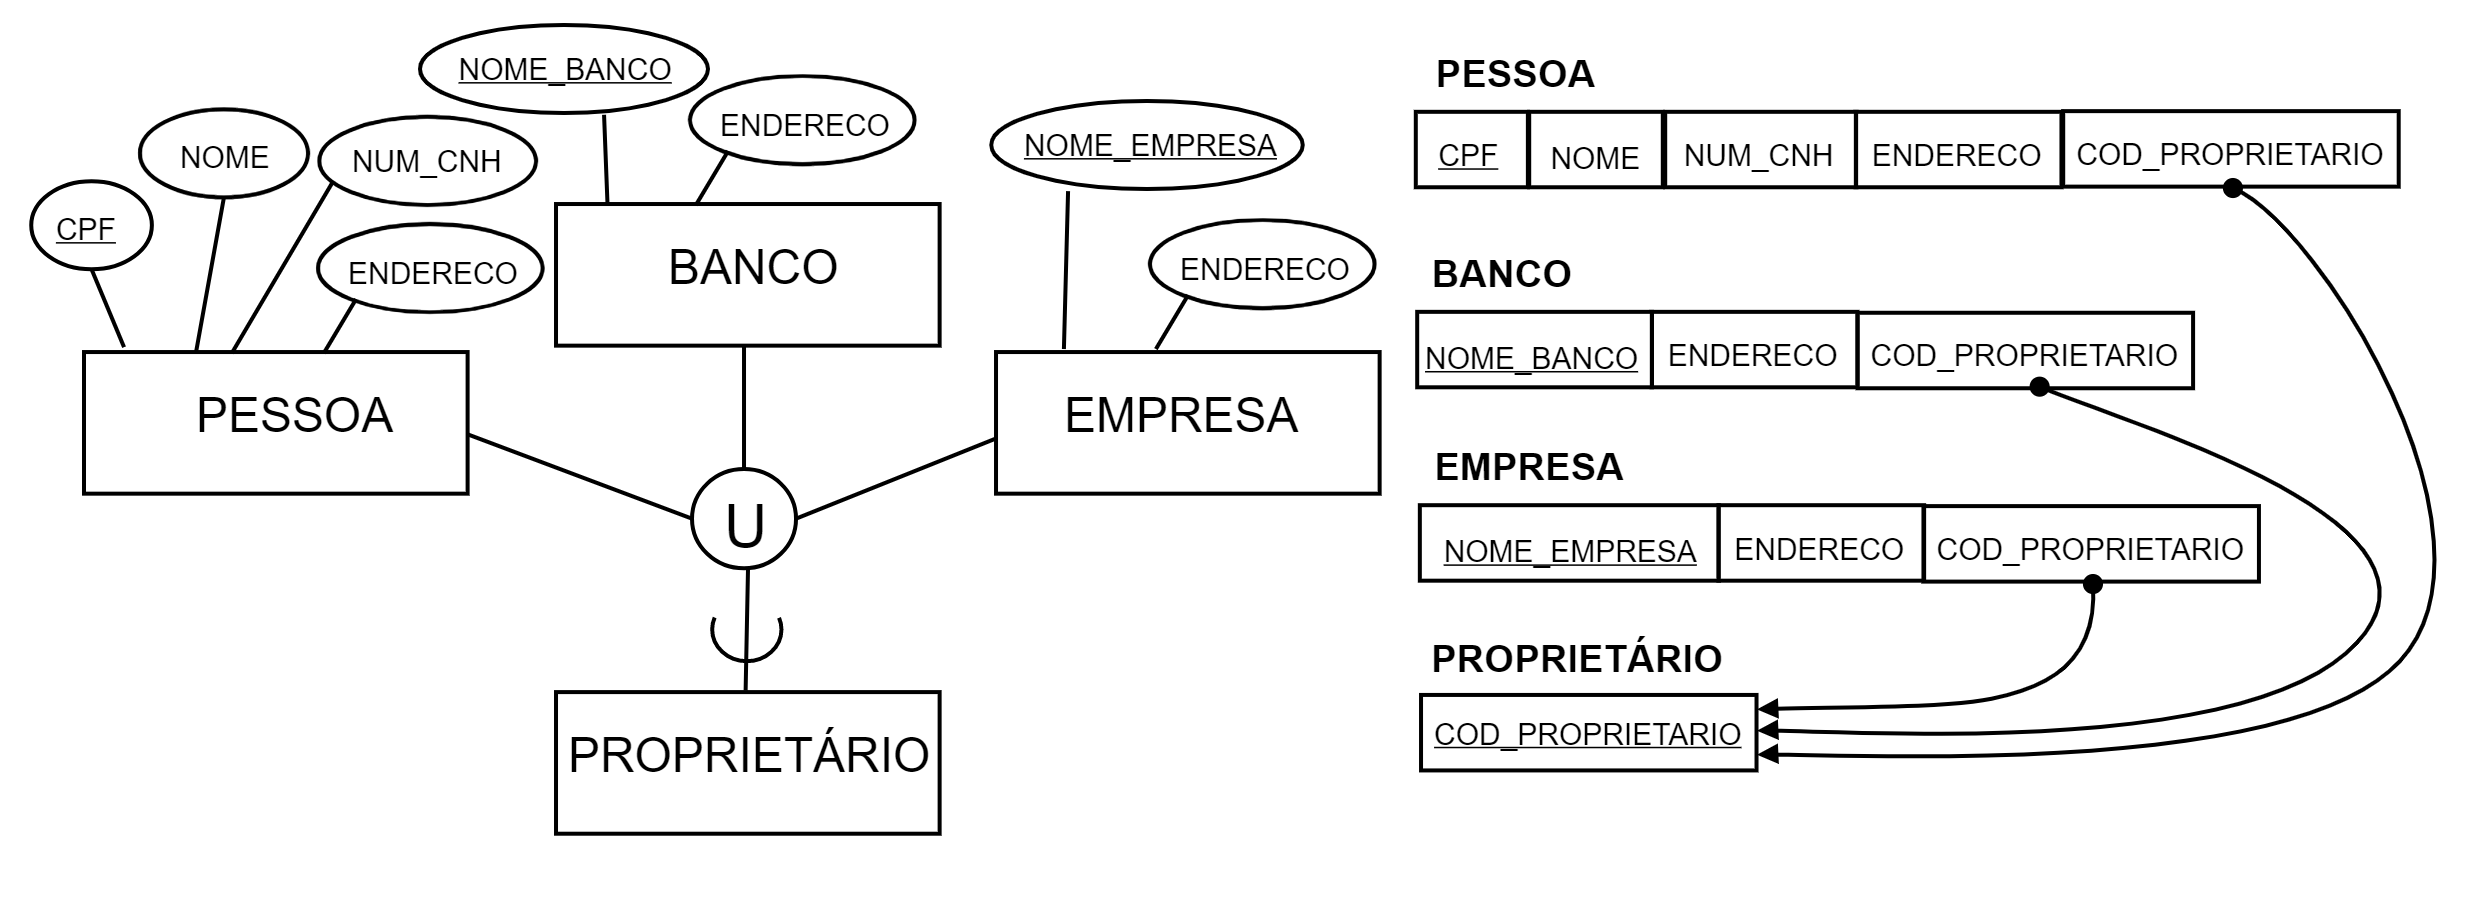
\includegraphics[scale=0.11]{Figuras/03_17.png}
\end{figure}
\end{ftst}

%==================================

\begin{ftst}{Praticando 1}{Mapeamento ER para relacional}

\begin{figure}
    \centering
    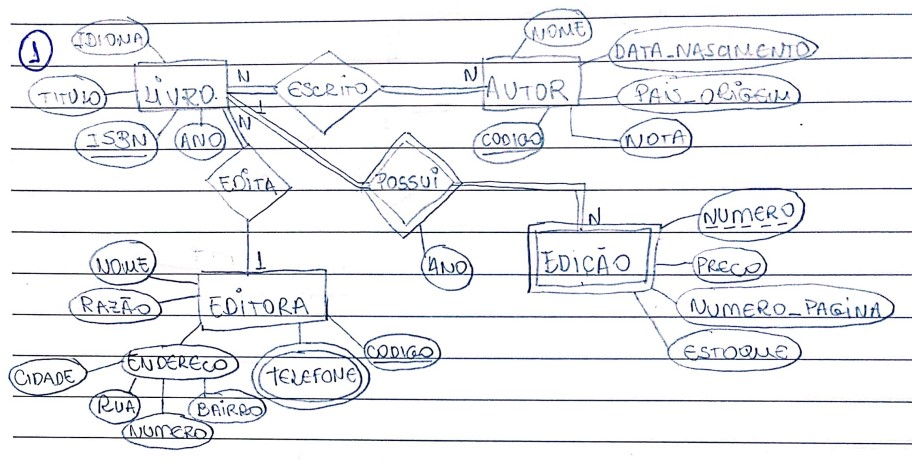
\includegraphics[scale=0.5]{Praticando_figuras/1.jpg}
\end{figure}
\end{ftst}

%==================================

\begin{ftst}{Praticando 2}{Mapeamento ER para relacional}

\begin{figure}
    \centering
    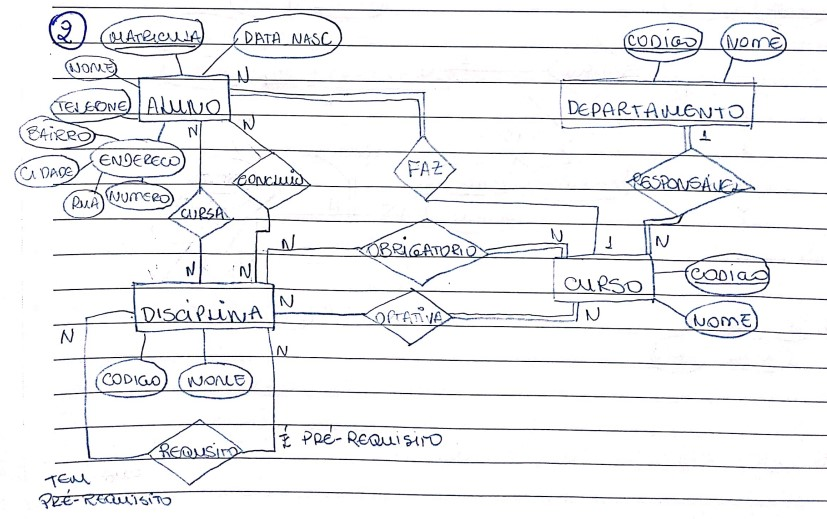
\includegraphics[scale=0.5]{Praticando_figuras/2.jpg}
\end{figure}
\end{ftst}

%==================================

\begin{ftst}{Praticando 3}{Mapeamento ER para relacional}

\begin{figure}
    \centering
    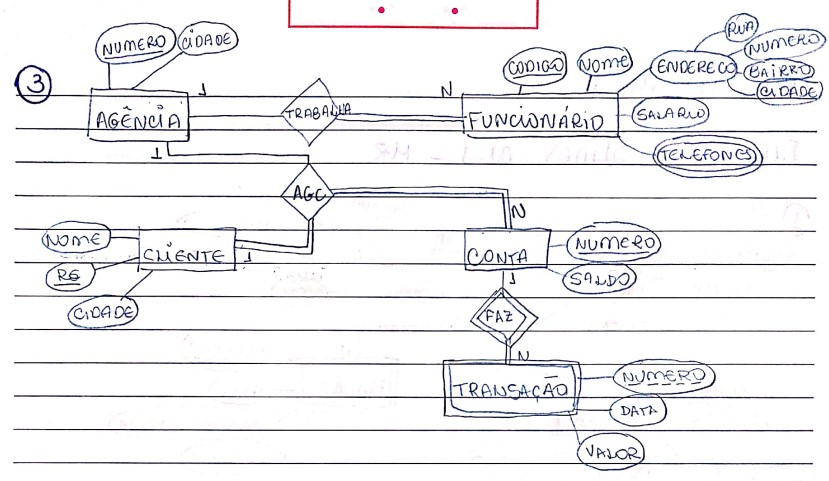
\includegraphics[scale=0.5]{Praticando_figuras/3.jpg}
\end{figure}
\end{ftst}

%==================================

\begin{ftst}{Praticando 4}{Mapeamento ER para relacional}

\begin{figure}
    \centering
    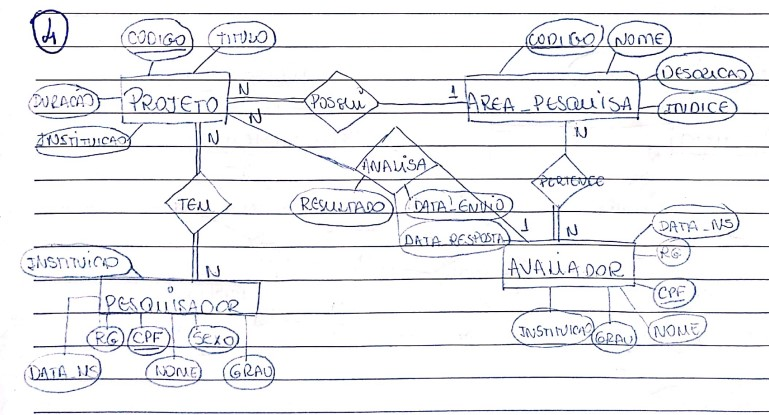
\includegraphics[scale=0.6]{Praticando_figuras/4.jpg}
\end{figure}
\end{ftst}

%==================================

\begin{ftst}{Praticando 5}{Mapeamento ER para relacional}

\begin{figure}
    \centering
    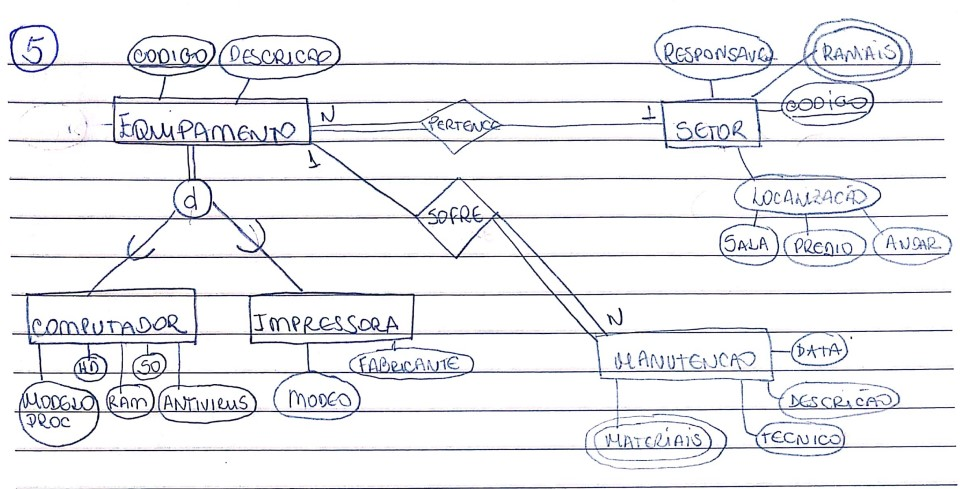
\includegraphics[scale=0.5]{Praticando_figuras/5.jpg}
\end{figure}
\end{ftst}

%==================================

\end{document}